%%
%% Beginning of file 'sample62.tex'
%%
%% Modified 2018 January
%%
%% This is a sample manuscript marked up using the
%% AASTeX v6.2 LaTeX 2e macros.
%%
%% AASTeX is now based on Alexey Vikhlinin's emulateapj.cls 
%% (Copyright 2000-2015).  See the classfile for details.

%% AASTeX requires revtex4-1.cls (http://publish.aps.org/revtex4/) and
%% other external packages (latexsym, graphicx, amssymb, longtable, and epsf).
%% All of these external packages should already be present in the modern TeX 
%% distributions.  If not they can also be obtained at www.ctan.org.

%% The first piece of markup in an AASTeX v6.x document is the \documentclass
%% command. LaTeX will ignore any data that comes before this command. The 
%% documentclass can take an optional argument to modify the output style.
%% The command below calls the preprint style  which will produce a tightly 
%% typeset, one-column, single-spaced document.  It is the default and thus
%% does not need to be explicitly stated.
%%
%%
%% using aastex version 6.2
\documentclass[twocolumn]{aastex62}

%% The default is a single spaced, 10 point font, single spaced article.
%% There are 5 other style options available via an optional argument. They
%% can be envoked like this:
%%
%% \documentclass[argument]{aastex62}
%% 
%% where the layout options are:
%%
%%  twocolumn   : two text columns, 10 point font, single spaced article.
%%                This is the most compact and represent the final published
%%                derived PDF copy of the accepted manuscript from the publisher
%%  manuscript  : one text column, 12 point font, double spaced article.
%%  preprint    : one text column, 12 point font, single spaced article.  
%%  preprint2   : two text columns, 12 point font, single spaced article.
%%  modern      : a stylish, single text column, 12 point font, article with
%% 		  wider left and right margins. This uses the Daniel
%% 		  Foreman-Mackey and David Hogg design.
%%  RNAAS       : Preferred style for Research Notes which are by design 
%%                lacking an abstract and brief. DO NOT use \begin{abstract}
%%                and \end{abstract} with this style.
%%
%% Note that you can submit to the AAS Journals in any of these 6 styles.
%%
%% There are other optional arguments one can envoke to allow other stylistic
%% actions. The available options are:
%%
%%  astrosymb    : Loads Astrosymb font and define \astrocommands. 
%%  tighten      : Makes baselineskip slightly smaller, only works with 
%%                 the twocolumn substyle.
%%  times        : uses times font instead of the default
%%  linenumbers  : turn on lineno package.
%%  trackchanges : required to see the revision mark up and print its output
%%  longauthor   : Do not use the more compressed footnote style (default) for 
%%                 the author/collaboration/affiliations. Instead print all
%%                 affiliation information after each name. Creates a much
%%                 long author list but may be desirable for short author papers
%%
%% these can be used in any combination, e.g.
%%
%% \documentclass[twocolumn,linenumbers,trackchanges]{aastex62}
%%
%% AASTeX v6.* now includes \hyperref support. While we have built in specific
%% defaults into the classfile you can manually override them with the
%% \hypersetup command. For example,
%%
%%\hypersetup{linkcolor=red,citecolor=green,filecolor=cyan,urlcolor=magenta}
%%
%% will change the color of the internal links to red, the links to the
%% bibliography to green, the file links to cyan, and the external links to
%% magenta. Additional information on \hyperref options can be found here:
%% https://www.tug.org/applications/hyperref/manual.html#x1-40003
%%
%% If you want to create your own macros, you can do so
%% using \newcommand. Your macros should appear before
%% the \begin{document} command.
%%


%% Other packages

\usepackage{xspace}
\usepackage{graphicx}
%\usepackage{epsfig}
\usepackage{times}
\usepackage{natbib}
\usepackage{amsfonts}
\usepackage{amsmath}
\usepackage{amsbsy}
\usepackage{bm}
\usepackage{hyperref}
\usepackage{url}
\usepackage[caption=false]{subfig}
\usepackage{microtype}
\usepackage{rotating}
\usepackage{booktabs}
\usepackage{threeparttable}
\usepackage{tabularx}
%\usepackage{subcaption}
\usepackage{minted}
\usepackage{listings}


\newcommand{\project}[1]{\textsl{#1}\xspace}
\newcommand{\fermi}{\project{Fermi}\xspace}
\newcommand{\rxte}{\project{RXTE}\xspace}
\newcommand{\nustar}{\project{NuSTAR}\xspace}

\newcommand{\Poisson}{\ensuremath{{\mathcal P}}\xspace}
\newcommand{\Uniform}{\ensuremath{{\mathcal U}}\xspace}
\newcommand{\bg}{\ensuremath{\mathrm{bg}}\xspace}
\newcommand{\word}{\ensuremath{\phi}\xspace}
\newcommand{\zsq}{\ensuremath{Z^2_n}\xspace}
%\newcommand{\stingray}{\mintinline{python}{stingray}\xspace}
\newcommand{\python}{\texttt{Python}\xspace}
\newcommand{\stingray}{\texttt{stingray}\xspace}
\newcommand{\astropy}{\texttt{astropy}\xspace}
\newcommand{\lightcurve}{\mintinline{python}{Lightcurve}\xspace}
\newcommand{\eventlist}{\mintinline{python}{EventList}\xspace}
\newcommand{\crossspectrum}{\mintinline{python}{Crossspectrum}\xspace}
\newcommand{\powerspectrum}{\mintinline{python}{Powerspectrum}\xspace}
\newcommand{\likelihood}{\mintinline{python}{Likelihood}\xspace}
\newcommand{\posterior}{\mintinline{python}{Posterior}\xspace}
\newcommand{\parest}{\mintinline{python}{ParameterEstimation}\xspace}

\newcommand{\hendrics}{\texttt{HENDRICS}\xspace}
\newcommand{\dave}{\texttt{DAVE}\xspace}



\usemintedstyle[python]{friendly}

%% Reintroduced the \received and \accepted commands from AASTeX v5.2
%\received{Dec 1, 2018}
%\revised{January 7, 2018}
%\accepted{\today}
%% Command to document which AAS Journal the manuscript was submitted to.
%% Adds "Submitted to " the arguement.
\submitjournal{ApJ}

%% Mark up commands to limit the number of authors on the front page.
%% Note that in AASTeX v6.2 a \collaboration call (see below) counts as
%% an author in this case.
%
%\AuthorCollaborationLimit=3
%
%% Will only show Schwarz, Muench and "the AAS Journals Data Scientist 
%% collaboration" on the front page of this example manuscript.
%%
%% Note that all of the author will be shown in the published article.
%% This feature is meant to be used prior to acceptance to make the
%% front end of a long author article more manageable. Please do not use
%% this functionality for manuscripts with less than 20 authors. Conversely,
%% please do use this when the number of authors exceeds 40.
%%
%% Use \allauthors at the manuscript end to show the full author list.
%% This command should only be used with \AuthorCollaborationLimit is used.

%% The following command can be used to set the latex table counters.  It
%% is needed in this document because it uses a mix of latex tabular and
%% AASTeX deluxetables.  In general it should not be needed.
%\setcounter{table}{1}

%%%%%%%%%%%%%%%%%%%%%%%%%%%%%%%%%%%%%%%%%%%%%%%%%%%%%%%%%%%%%%%%%%%%%%%%%%%%%%%%
%%
%% The following section outlines numerous optional output that
%% can be displayed in the front matter or as running meta-data.
%%
%% If you wish, you may supply running head information, although
%% this information may be modified by the editorial offices.
\shorttitle{\stingray: A Modern \python\ Library For Spectral Timing}
\shortauthors{Huppenkothen et al.}
%%
%% You can add a light gray and diagonal water-mark to the first page 
%% with this command:
% \watermark{text}
%% where "text", e.g. DRAFT, is the text to appear.  If the text is 
%% long you can control the water-mark size with:
%  \setwatermarkfontsize{dimension}
%% where dimension is any recognized LaTeX dimension, e.g. pt, in, etc.
%%
%%%%%%%%%%%%%%%%%%%%%%%%%%%%%%%%%%%%%%%%%%%%%%%%%%%%%%%%%%%%%%%%%%%%%%%%%%%%%%%%

%% This is the end of the preamble.  Indicate the beginning of the
%% manuscript itself with \begin{document}.

\begin{document}

\title{\stingray: A Modern \python\ Library For Spectral Timing}

%% LaTeX will automatically break titles if they run longer than
%% one line. However, you may use \\ to force a line break if
%% you desire. In v6.2 you can include a footnote in the title.

%% A significant change from earlier AASTEX versions is in the structure for 
%% calling author and affilations. The change was necessary to implement 
%% autoindexing of affilations which prior was a manual process that could 
%% easily be tedious in large author manuscripts.
%%
%% The \author command is the same as before except it now takes an optional
%% arguement which is the 16 digit ORCID. The syntax is:
%% \author[xxxx-xxxx-xxxx-xxxx]{Author Name}
%%
%% This will hyperlink the author name to the author's ORCID page. Note that
%% during compilation, LaTeX will do some limited checking of the format of
%% the ID to make sure it is valid.
%%
%% Use \affiliation for affiliation information. The old \affil is now aliased
%% to \affiliation. AASTeX v6.2 will automatically index these in the header.
%% When a duplicate is found its index will be the same as its previous entry.
%%
%% Note that \altaffilmark and \altaffiltext have been removed and thus 
%% can not be used to document secondary affiliations. If they are used latex
%% will issue a specific error message and quit. Please use multiple 
%% \affiliation calls for to document more than one affiliation.
%%
%% The new \altaffiliation can be used to indicate some secondary information
%% such as fellowships. This command produces a non-numeric footnote that is
%% set away from the numeric \affiliation footnotes.  NOTE that if an
%% \altaffiliation command is used it must come BEFORE the \affiliation call,
%% right after the \author command, in order to place the footnotes in
%% the proper location.
%%
%% Use \email to set provide email addresses. Each \email will appear on its
%% own line so you can put multiple email address in one \email call. A new
%% \correspondingauthor command is available in V6.2 to identify the
%% corresponding author of the manuscript. It is the author's responsibility
%% to make sure this name is also in the author list.
%%
%% While authors can be grouped inside the same \author and \affiliation
%% commands it is better to have a single author for each. This allows for
%% one to exploit all the new benefits and should make book-keeping easier.
%%
%% If done correctly the peer review system will be able to
%% automatically put the author and affiliation information from the manuscript
%% and save the corresponding author the trouble of entering it by hand.

\correspondingauthor{Daniela Huppenkothen}
\email{dhuppenk@uw.edu}

\author[0000-0002-1169-7486]{Daniela Huppenkothen}
\affil{DIRAC Institute, \\
Department of Astronomy, \\ 
University of Washington, \\
3910 15th Ave NE, Seattle, WA 98195}
\nocollaboration

\author[0000-0002-4576-9337]{Matteo Bachetti}
\affiliation{INAF-Osservatorio Astronomico di Cagliari, \\
 via della Scienza 5, \\
 I-09047 Selargius (CA), Italy}
\nocollaboration

\author[0000-0002-5041-3079]{Abigail L. Stevens}
\affiliation{Department of Physics \& Astronomy, Michigan State University, 567 Wilson Road, East Lansing, MI 48824, USA}
\affiliation{Department of Astronomy, University of Michigan, 1085 South University Avenue, Ann Arbor, MI 48109, USA}\nocollaboration

\author{OTHERS!}
\altaffiliation{}

%% Note that the \and command from previous versions of AASTeX is now
%% depreciated in this version as it is no longer necessary. AASTeX 
%% automatically takes care of all commas and "and"s between authors names.

%% AASTeX 6.2 has the new \collaboration and \nocollaboration commands to
%% provide the collaboration status of a group of authors. These commands 
%% can be used either before or after the list of corresponding authors. The
%% argument for \collaboration is the collaboration identifier. Authors are
%% encouraged to surround collaboration identifiers with ()s. The 
%% \nocollaboration command takes no argument and exists to indicate that
%% the nearby authors are not part of surrounding collaborations.

%% Mark off the abstract in the ``abstract'' environment. 
\begin{abstract}
% This abstract could be more exciting, I think.
This paper describes the design, implementation and usage of \stingray, a library in \python built to perform time series analysis and related tasks on astronomical light curves. 
Its core functionality comprises a range of Fourier analysis techniques commonly used in Spectral Timing, as well as extensions for analysing pulsar data, simulating data sets, and statistical modelling. 
Its modular build allows for easy extensions and we aim for the library to be a platform for the implementation of future spectral timing techniques.  
Here, we describe the overall vision and framework, as well as core functionality, extensions and connections to high-level command-line and graphical interfaces.
The code is well-tested, with a test coverage of currently 95\%, and is accompanied by extensive API documentation as well as a set of step-by-step tutorials.
\end{abstract}

%% Keywords should appear after the \end{abstract} command. 
%% See the online documentation for the full list of available subject
%% keywords and the rules for their use.
\keywords{methods:statistics}

%% From the front matter, we move on to the body of the paper.
%% Sections are demarcated by \section and \subsection, respectively.
%% Observe the use of the LaTeX \label
%% command after the \subsection to give a symbolic KEY to the
%% subsection for cross-referencing in a \ref command.
%% You can use LaTeX's \ref and \label commands to keep track of
%% cross-references to sections, equations, tables, and figures.
%% That way, if you change the order of any elements, LaTeX will
%% automatically renumber them.
%%
%% We recommend that authors also use the natbib \citep
%% and \citet commands to identify citations.  The citations are
%% tied to the reference list via symbolic KEYs. The KEY corresponds
%% to the KEY in the \bibitem in the reference list below. 

\section{Introduction} \label{sec:intro}

Variability is one of the key diagnostics in understanding the underlying physics of the dynamics and emission processes from astronomical objects. 
The detection of periodic variations in the radio flux of certain objects has led to the ground-breaking discovery of pulsars [REF!]. Similarly, accurately describing of dips in stellar light curves has led to the discovery of thousands of exoplanets [REF!]. 
In high-energy astrophysics, particularly the study of black holes and neutron stars, the scientific developments of recent years have brought a growing understanding that time and wavelength are intricately linked [REF]. 
Different spectral components react differently to changes in accretion rate and dynamics, leading to time lags, correlated variability and higher-order effects [REF]. 
This has led to the study of accretion disks, in particular those of Active Galactic Nuclei (AGN), via reverberation mapping [REF], and probes of the accretion disk geometry using the energy-dependence of quasi-periodic oscillations in stellar-mass black holes [REF Adam's paper]. 
Understanding how the emission at various wavelengths changes with time is crucial for testing and expanding our understanding of General Relativity in the strong gravity limit, the dense matter equation of state and other fundamental questions in astrophysics [REF].
In X-rays, there is now a wealth of data sets of variable objects from missions such as the \textit{Rossi X-ray Timing Explorer} (\rxte; REF), the \textit{Nuclear Spectroscopic Telescope Array} (\nustar; REF), and more recently the Neutron Star Interior Composition Explorer (\textit{NICER}; REF). In addition, planned missions such as the Advanced Telescope for High-ENergy Astrophysics (\textit{Athena}; REF) will produce data sets of unprecedented size and complexity, motivating the need for scalable algorithms and the well-tested, open-source software described in this manuscript.

The paper layout is as follows: 
In Section \ref{sec:data}, we very briefly describe the data sets being used in this paper to showcase the implemented methods. In Section \ref{sec:vision}, we lay out the overall vision, followed by a description of the general package structure. The package's core functionality is shown in more detail in Section \ref{sec:core}, where we introduce basic classes for generating light curves and Fourier spectra of various types.
In Sections \ref{sec:modeling}, \ref{sec:simulator} and \ref{sec:pulsar}, we lay out the submodules allowing modelling Fourier products, simulating light curves from stochastic processes, and pulsar analysis, respectively.
Sections \ref{sec:hendrics} and \ref{sec:dave} detail existing connections to the command-line interface and a graphical user interface, respectively, which are currently being developed in parallel to \stingray. 
Finally, in Sections \ref{sec:development} and \ref{sec:future} we lay out the development process, testing and documentation environments as well as our future development plans. 
In each section, we present examples of the functionality described based on either simulated or real-world data sets. Note that we intentionally omit code examples in this manuscript in order to preserve long-term accuracy. All code to reproduce the figures in this paper is available online\footnote{\url{https://github.com/StingraySoftware/stingraypaper}}, and a full suite of up-to-date tutorials is also available\footnote{\url{https://github.com/StingraySoftware/notebooks}}.

\section{Data}
\label{sec:data}
Throughout the paper, we use real X-ray observations of compact objects to demonstrate the functionality of the software in this package. Here, we give brief introductions into the observations used and the data reduction processes applied before using the resulting event files and time series with \stingray.

\subsection{GX 339-4}
\label{sec:gx339}

GX 339--4 is a stellar black hole in a low-mass X-ray binary \citep{Hynesetal03}. 
The black hole has a lower mass limit of $\sim$\,7\Msun\ \citep{MunozDariasetal08} and possibly a near-maximal spin \citep{Ludlametal15}. 
The system also likely has a low binary orbit inclination; it has been constrained to $37\degrees <i\lesssim 60\degrees$ from optical and X-ray observations \citep{Heidaetal17, Zdziarskietal98}, and spectral modelling by \citet{WangJietal18} estimates $i\approx 40\degrees$.
For this example we use an Rossi X-ray Timing Explorer (RXTE; \citealt{Bradtetal93}) Proportional Counter Array (PCA; \citealt{Jahodaetal96}) observation in NASA's High Energy Astrophysics Science Archive Research Center (HEASARC) from the 2010 outburst of GX 339--4 \citep{Yamaokaetal10}.
We are using observation ID 95409-01-15-06 taken from UT 2010-04-22 23:36:52 to UT 2010-04-23 00:01:10.
This observation was taken in 64-channel event mode with $122\,\mu$s time resolution (\texttt{E\_125us\_64M\_0\_1s}).
The following filtering criteria were used to obtain Good Time Intervals (GTIs): Proportional Counter Unit (PCU) 2 is on, two or more PCUs are on, elevation angle $>$\,10\degrees, and target offset $<$\,0.02\degrees. 
Time since the South Atlantic Anomaly passage was not filtered on. 

\subsection{Hercules X-1}
\label{sec:herx1}

Hercules X-1 (Her X-1) is a well-known persistent X- ray binary pulsar with a period of $P = 1.23 \mathrm{s}$ \citep{tananbaum1972} in a binary system with a $\sim 2.2 M_\odot$ stellar companion HZ Herculis \citep{davidsen1972,forman1972,bahcall1972,reynolds1997,leahy2014} with an orbital period of $P_\mathrm{orb}=1.7\,\mathrm{days}$ and super-orbital variations on a $\sim$35-day timescale \citep{giacconi1973,scott1999,igna2011}. The companion's type varies between late-type A and early-type B with orbital phase \citep{anderson1994,cheng1995}. 
For this work, we considered one of several observations of Her X-1 with the \textit{Nuclear Spectroscopic Telescope Array} (\nustar; REF). The observation was taken from UT 2012-09- 19 to UT 2012-09-20 and was one among several used by \citep{Fuerst13} to characterize the cyclotron resonance scattering features in the spectrum of the source. We downloaded the observation directory for observation ID 30002006002 from the HEASARC and used the FTOOL barycorr on the L2 cleaned science event files (file name ending with \verb|01_cl.evt|) to correct the photon arrival times to the solar system barycenter. For our analysis, we considered photons from 3 to 79 keV at most 50?? from the nominal position of the source, extracted from the two identical Focal Plane Modules A and B (FPMA and FPMB, respectively) onboard the spacecraft. We used a total of 32.67ks of good time intervals (GTIs), only selecting intervals longer than 10s. 

%\subsection{Simulated Data}


%\begin{table}[hbtp]
%\footnotesize
%\caption{Parameters for the simulated data set}
%\begin{threeparttable} 
%\begin{tabularx}{8.5cm}{p{2.5cm}p{4.0cm}p{2.0cm}}
%\toprule
%\bf{Parameter} & \bf{Description} &\bf{Value} \\ \midrule
%$A_{\mathrm{PL}}$ & Power law amplitude & $0.1$ \\
%$\alpha$ & Power law spectral index & 1.0 \\
%$A_{\mathrm{QPO}}$ & QPO amplitude &  $1.0$ \\
%$\nu_0$ & QPO centroid frequency & $2.0 \,\mathrm{Hz}$ \\
%$\gamma$ & QPO full width at half-maximum &$1 \,\mathrm{Hz}$ \\
% \bottomrule
%\end{tabularx}
%   \begin{tablenotes}
%      \item{}
%\end{tablenotes}
%\end{threeparttable}
%\label{table:parameters}
%\end{table}

% To showcase much of the functionality in the following chapters, we assume a process producing a power spectrum with an intrinsic spectrum comprising a power law and a quasi-periodic oscillation, approximated by a Lorentzian function (Figure \ref{fig:lightcurve}, left panel):

%\[
%P(\nu) = A_{\mathrm{PL}} \nu^{\alpha} + \frac{A \gamma^2}{\gamma^2 + (\nu - \nu_0)^2} \, .
%\]

%We use the algorithm from \citet{timmer1995} to generate a light curve with a time resolution of $\delta t = 0.05\,\mathrm{s}$ and a length of $15.36 \,\mathrm{ks}$, amounting to $307200$ data points. The power law has a spectral index of $\alpha = 1.0$, the QPO a centroid frequency of $2 \,\mathrm{Hz}$. The generated light curve has a mean count rate of $400\,\mathrm{counts/s}$ and a fractional rms amplitude of $\mathrm{rms}_\mathrm{frac} = 0.3$. Because the resulting light curve will follow Gaussian uncertainties, we simulate photon counting statistics by drawing from a Poisson distribution for every bin with a rate parameter equal to the simulated flux in that bin. 
%The remaining parameters can be found in Table \ref{tab:simdata}\footnote{The full code to reproduce all figures in this paper can be found at \url{https://github.com/stingraysoftware/stingraypaper}}. 


%%% GENERAL PACKAGE FRAMEWORK %%%%%%%%%%%%%%%%%%%%%%%%%%%%%%%%%%%%%%%%%%%%%%%%%%%%%%%%%%%%%%%%%%%%%%%%%%%%%

\section{Vision and General Package Framework}
\label{sec:vision}

Despite decades of research, the field of spectral timing in high-energy astrophysics is fragmented in terms of software; there is no commonly accepted, up-to-date framework for the core data analysis tasks involved in (spectral) timing. Code is generally siloed within groups, leading to a general lack of reproducibility of scientific results. Additionally, the lack of fully open-source tools constitutes a significant barrier to entry for researchers new to the field, since it effectively requires anyone not part of collaborations with an existing private code base to write their own software from scratch. 
The NASA library \texttt{xronos} is, to our knowledge, the only significant open-source library in this field, and has several shortcomings. 
In particular, it performs only a few of the most basic tasks, and it has not been maintained since 2004. 
This dearth of accessible tools motivated the development of \stingray, a library built entirely in \python and based on \astropy functionality, to address the lack of well-tested, well-documented software for spectral timing. 
\stingray aims to make many of the core Fourier analysis tools used in timing analysis available to a large range of researchers while providing a common platform for new methods and tools as they enter the field. 
It includes the most relevant functionality in its core package, while extending that functionality in its subpackages in several ways, allowing for easy modeling of light curves and power spectra, simulation of synthetic data sets and pulsar timing. 

Its core idea is to provide time series analysis methods in an accessible, well-tested way, built as a series of object-oriented modules. In practice, data analysis requirements are varied and depend on the type of data, the wavelength the observation was taken at, and the object being observed. With this in mind, \stingray does not aim to provide full-stack data analysis workflows; rather, it provides the core building blocks for users to build such workflows themselves, based on the specific data analysis requirements of their source and observation. 
The modularity of its classes allows for easy incorporation of existing \stingray functionality into larger data analysis workflows and pipelines, while being easily extensible for cases that the library currently does not cover. 

\stingray separates out core functionality from several more specialized tasks based on those core classes and functions. Constructs related to data products as well as Fourier transforms of the data (e.g.\ power spectra, cross spectra, time lags, and other spectral timing products) are considered core functionality, as are some utility functions and classes, for example related to Good Time Interval calculations. 

This core functionality is extended in various ways in currently three subpackages. The \mintinline{python}{modeling} subpackage (see also Section \ref{sec:modeling} provides a framework for modelling light curves and Fourier spectra with parametric functions. Based on this framework, it allows users to search efficiently for (quasi-)periodic oscillations in light curves with stochastic variability, and provides convenience functions to aid standard tasks like fitting Lorentzian functions to power spectra. 

The subpackage \mintinline{python}{simulator} (Section \ref{sec:simulator}) provides important functionality to allow efficient simulation of time series from a range of stochastic processes. This includes simulation of light curves from power spectral models as well as the use of transfer functions to introduce time lags and higher-order effects. 

Finally, the subpackage \mintinline{python}{pulsar} implements a range of methods particularly useful for period searches in pulsars. While no other sub-packages are currently under construction, we will implement new sub-packages based on core functionality as required. 


\stingray is formally hosted as part of a GitHub [REF?] organization called \textit{StingraySoftware}, which also hosts the website, documentation, a repository with tutorial notebooks, this manuscript, as well as the two related software packages. \stingray is designed to be used both as a standalone package, but is also at the core of two other software packages currently under development: \hendrics (\citealt{hendrics}; see also Section \ref{sec:hendrics}) provides pre-built data analysis workflows using \stingray core functionality. These workflows are accessible from the command line and are provided for some common data types and data analysis tasks. \dave\footnote{\url{https://github.com/StingraySoftware/dave}} (see also Section \ref{sec:dave}) provides a Graphical User Interface on top of \stingray to allow for easy interactive exploratory data analysis.
 
As of v0.1, \stingray is entirely written in Python, and its core functionality depends exclusively on \texttt{numpy} \citep{numpy}, \texttt{scipy} \citep{scipy} and \texttt{astropy} \citep{astropy}, with optional plotting functionality supplied by \texttt{matplotlib} \citep{matplotlib} . The \texttt{modeling} subpackage optionally uses sampling methods supplied by \texttt{emcee} \citep{emcee}, some functionality implemented in \texttt{statsmodels}, and plotting using \texttt{corner} \citep{corner}. The \texttt{pulse} subpackage optionally allows for just-in-time compilation using \texttt{numba} \citep{numba} for computational efficiency.

This paper describes \stingray v0.1, released on 2018-02-12. 
As with most open-source packages, \stingray is under continuous development and welcomes contributions from the community.

%%% CORE FUNCTIONALITY %%%%%%%%%%%%%%%%%%%%%%%%%%%%%%%%%%%%%%%%%%%%%%%%%%%%%%%%%%%%%%%%%%%%%%%%%%%%%%%%%%%%%%%%%

\section{Core Functionality}
\label{sec:core}

\stingray imports its core functions and classes from the top level package. 
These classes define the basic data structures such as light curves and cross- as well as power spectra that are used in much of the higher-level functionality provided in the sub-packages. 
Additionally, it incorporates a number of utilities for dealing with Good Time Intervals (GTIs) as well as input and output of data sets. 
\subsection{The \texttt{Lightcurve} class}
\label{sec:lightcurve}

%\begin{figure}[htbp]
%\begin{center}
%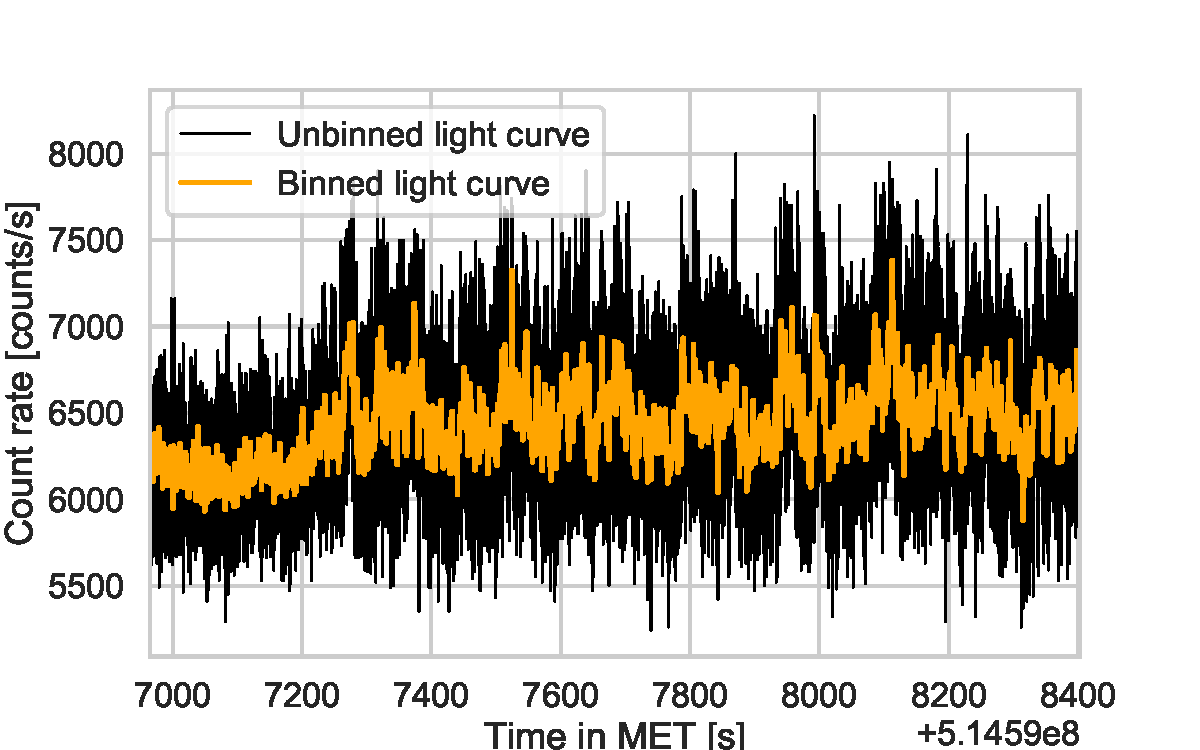
\includegraphics[width=0.5\textwidth]{../figures/example_lc.pdf}
%\caption{An example light curve of the black hole X-ray binary GRS 1915+105, taken with the \textit{Rossi} X-ray Timing Explorer's Proportional Counter Array (PCA) in the $\rho$ state [REF]. This is a short, $250\,\mathrm{s}$ segment of a longer data, part of a longer observation (shown in Figure \ref{fig:psd}, panel (a) below). In black, the unbinned Standard 2 light curve at $dt = 0.125\mathrm{s}$ time resolution. In orange, we show a rebinned light curve with a time resolution of $dt = 1.25\mathrm{s}$.}
%\label{fig:lc}
%\end{center}
%\end{figure}

We expect \stingray to be used largely on data sets of two forms: (1) event data (i.e. recordings of arrival times of individual photons) or (2) binned light curves. 

The majority of methods in \stingray use binned light curves, which we thus currently consider the default format. The \lightcurve class defines a basic data structure to store binned light curves. Its features include arrays describing time bins and associated (flux or counts) measurements, the number of data points in the light curve, the time resolution and the total duration of the light curve. For unevenly sampled light curves, the time resolution \texttt{dt} will be defined as the median difference between time bin midpoints. Users can pass uncertainties for measurements directly, or pass a string defining the statistical distribution of the data points for automatic calculation. By default, a Poisson distribution is assumed, appropriate for binned event data. 

There are two ways to generate a \texttt{Lightcurve} object: in the standard case, the instrument has recorded a binned time series of $N$ pairs of time stamps and count (rate) or flux values, $\{t_k, c_k \}_{k=1}^{N}$. In this case, one can simply instantiate a \texttt{Lightcurve} object with the keywords \texttt{time} and \texttt{counts} (and optionally set \texttt{use\_counts=False} when the input is in units of counts per second). In cases where the native data format is events (e.g.\ photon arrival times) it is possible to use the static method \texttt{Lightcurve.make\_lightcurve}, passing the array of events as well as a time resolution \texttt{dt} to create a new light curve from the events.

Various operations are implemented for class \lightcurve. Custom behaviour of the $+$ and $-$ operators allows straightforward addition and subtraction of light curves from one another. Assuming the light curves have the same time bins, the $+$ and $-$ operators will add or subtract the flux or counts measurements, respectively, and return a new \lightcurve\ object with the results. Other common operations implemented include time-shifting the light curve by a constant factor, joining two light curves into a single object, truncating a light curve at a certain time bin, and input/output operations to read or write objects from/to disk in various formats (HDF5, FITS and ASCII are currently supported). For light curves that do not have consecutive time bins, there is a sorting operations, as well as the option to sort the light curve by the ascending or descending flux or counts. 

We provide support for Good Time Intervals (GTIs) in many methods and implement rebinning the light curve to a new time resolution exceeding the native resolution of the data (interpolation to a finer resolution is currently not supported). In Figure \ref{fig:psd} (left panel), we show an example observation of GX 339-4 as taken with with \rxte.

Other functionality on light curves includes rebinning to a new time resolution, which must be lower than the previous time resolution (i.e.\ interpolation is not implemented; see also Figure \ref{fig:psd}, left panel, for an example). 
\lightcurve objects can also be joined, truncated and sorted by time or counts. Finally, \stingray implements basic methods for plotting (useful for a quick look at the data), as well as reading and writing into various formats (currently FITS, HDF5 and ASCII).

\begin{figure*}[htbp]
\begin{center}
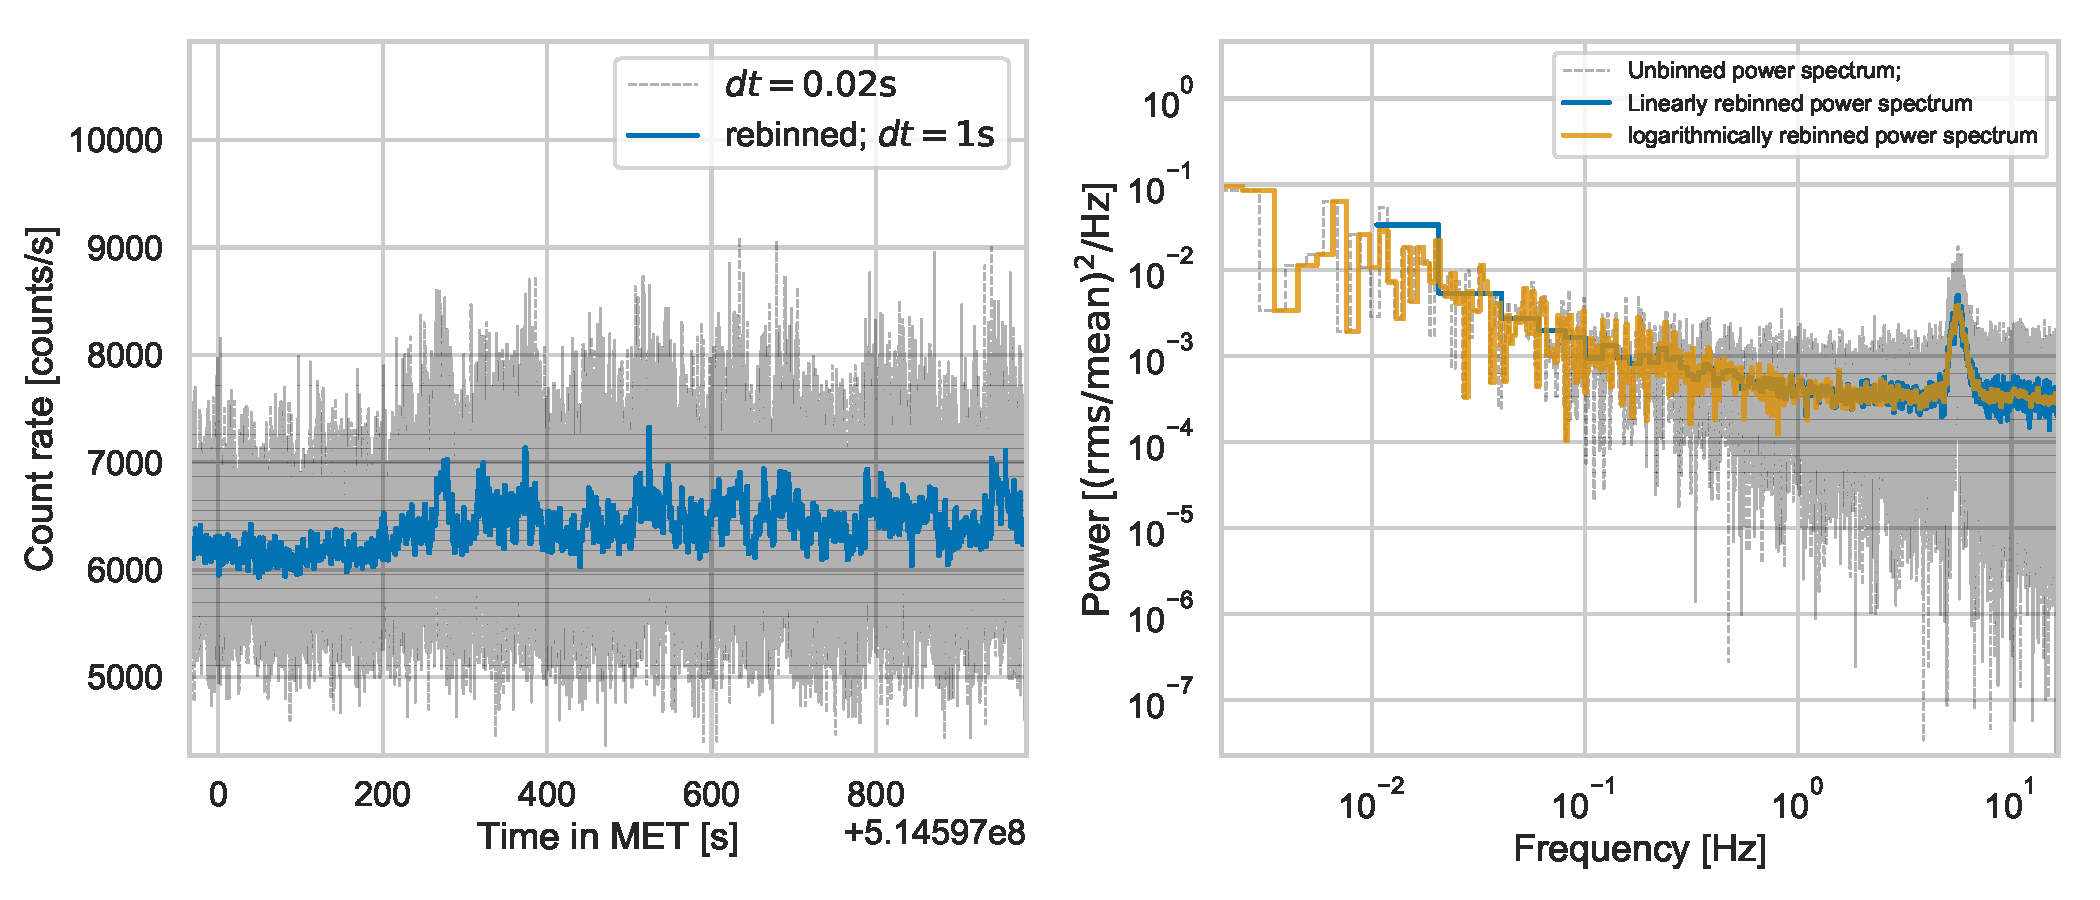
\includegraphics[width=\textwidth]{../figures/example_lc_ps.pdf}
\caption{Left panel: A $\sim 1 \mathrm{ks}$ observation of the black hole X-ray binary GX 339-4 observed with \rxte. Details of the observation can be found in Section \ref{sec:gx339}. In grey, we show the light curve produced by binning the events into $0.02\,\mathrm{s}$ bins. The blue line corresponds to the rebinned light curve at $dt = 1.0\,\mathrm{s}$. Right panel: we show the power spectrum calculated from the light curve in the left panel (grey), as well as a version of the same power spectrum that has been linearly rebinned in frequency (blue), and a version that was logarithmically rebinned (orange).}
\label{fig:psd}
\end{center}
\end{figure*}

\subsection{The \texttt{Events} class}

At short wavelengths, data is largely recorded as \textit{photon events}, where arrival times at the detector are recorded for each photon independently, along with a number of other properties of the event (for example an energy channel in which the photon was recorded in, which can be transformed to a rough estimate of the energy of the original photon arriving at the detector).

Even for a single instrument, there are often multiple data formats and types of data recorded, resulting in a plethora of data formats and internal schema to how data is stored within the FITS files distributed to the community. \stingray implements a basic \eventlist class that acts as a container for basic event data, but does not aim to encompass all data types of all current (and future) instruments entirely. Instead, it aims to abstract away from instrument-specific idosyncrasies as much as possible and remain mission-agnostic. In its basic form, it takes arrays with time stamps and optionally corresponding photon energies as input, and implements a set of basic methods. Similarly to \lightcurve, it provides basic input/output (I/O) functionality in the form of \texttt{read} and \texttt{write} methods as well as a method to join event lists, which can be particularly useful when data is recorded in several independent detector, as is common for several current and future X-ray missions. The \verb|to_lc| method provides straightforward connection to create a \lightcurve directly out of an \eventlist object. In return, it is possible to create an \eventlist out of a \lightcurve object using the \verb|from_lc|. The latter will create $N_i$ events, each with a time stamp equation to the time bin $t_i$, where $N_i$ is the number of counts in bin $i$ (event lists are, by their very definition only a useful data product if the light curve used to simulate comes from photon counting data in the first place). 
It is possible to simulate more physically meaningful photon events from a given light curve and energy spectrum using the \verb|simulate_times| and \verb|simulate_energies| methods, which employ a combination of interpolation and rejection sampling to accurately draw events from the given light curve and spectrum.


\subsection{Cross Spectra and Power Spectra}
\label{sec:csps}

The cross spectrum and the power spectrum\footnote{In the signal processing literature, generally a distinction is made between the power spectrum, which
describes the process at the source generating variable time series, and the periodogram, which denotes a realization of said power spectrum, i.e. the time series we actually observe. While the products generated by \stingray generally fall into the latter category, the astronomy literature usually denotes them by the term power spectrum. We follow this convention here as we do within the software package itself.} are closely related (for a pedagogical introduction into Fourier analysis, see \citealt{vanderklis1989}; see also \citealt{uttley2014} for a recent review of spectral timing techniques). Computing the cross spectrum requires two evenly sampled time series $\mathbf{y}_1 = \{y_{1,i}\}_{i=1}^{N} $ and $\mathbf{y}_2 =  \{y_{2,i}\}_{i=1}^{N}$ taken simultaneously at exactly the same time intervals $\{t_i \}_{i=1}^N$. Under this assumption, one may then compute the discrete Fourier transform of each time series, $\mathcal{F}_1$ and $\mathcal{F}_2$ independently, and multiple the $\mathcal{F}_1$ with $\mathcal{F}^{*}_2$, i.e. the Fourier transform of the first time series with the \textit{complex conjugate} of the Fourier transform of $\mathbf{y}_2$. 

Because the power spectrum is defined as the square of the real part of the Fourier amplitudes of a single, evenly sampled time series, it can be formulated as the special case of the cross spectrum where $\mathbf{y}_1 = \mathbf{y}_2$. In \stingray, we implement a class \crossspectrum, which takes two \lightcurve objects as input and internally calculates the complex cross spectrum in one of a number of common normalizations.  Because many of the internal calculations are the same, the class \powerspectrum is implemented as a subclass of \crossspectrum, but takes only a single \lightcurve object instead of two. 

There are several popular normalizations for the real part of the cross spectrum as well as the power spectrum implemented in \stingray: the \textit{Leahy normalization} \citep{leahy1983} is defined such that for simple white noise, the power spectrum will follow a $\chi^2$ distribution with $2$ degrees of freedom around a mean value of $2$. It is particularly useful for period searches, because the white noise level is well understood and always the same (but be aware that detector effects like dead time can distort the power spectrum in practice \citep{Bachetti+15}).
For light curves with complex variability patterns, and especially understanding how these patterns contribute to the overall variance observed, the \textit{fractional rms normalization} \citep{belloni1990,miyamoto1992}  or the \textit{absolute rms normalization} \citep{uttley2001} may be more appropriate choices. 

%These normalizations can be set when instantiating a \crossspectrum or \powerspectrum object using the keyword argument \texttt{norm}, e.g.
%\begin{minted}{python}
%ps = Powerspectrum(lc, norm="leahy")
%\end{minted}
%\noindent Setting \mintinline{python}{norm="none"} will return the raw, unnormalized powers. 
The classes \crossspectrum and \powerspectrum share most of the implemented methods, except where otherwise noted. Both classes include methods to rebin cross- and power spectra. Linear rebinning is implemented analogously to the method in class \lightcurve. Additionally, logarithmic binning is implemented in the method \mintinline{python}{rebin_log} in such a way that the bin width at a given frequency increases a fraction of the previous bin width:

\[
d\nu_{i+1} = d\nu_{i} (1 + f) \; ,
\]

\noindent where $f$ is some constant factor by which the frequency resolution increases, often $f = 0.01$. 

In the case of the cross spectrum, it is also possible to calculate the time lag, defined as

\[
\tau_j = \frac{\phi_j}{2\pi\nu_j} \; 
\]

\noindent for a phase angle $\phi_j$ derived from the imaginary component of the complex cross spectrum, and a mid-bin frequency $\nu_j$. Similarly, it is possible to calculate the coherence \citep{vaughan1997,nowak1999} from the cross spectrum, defined as 

\begin{equation}
c_j = \frac{C_{xy,j}}{C_{x,j} C_{y,j}} \; . 
\end{equation}

\noindent Here, $C_{xy,j}$ corresponds to the real part of the unnormalized cross spectrum, and $C_{x,j}$ and $C_{y,j}$ correspond to the analogous squared amplitudes of the power spectrum for each individual light curve. 

Classical period searches are often formulated as outlier detection problems from an expected statistical distribution. Assuming the signal is sufficiently coherent such that all of the signal power is concentrated in one bin, one may calculate the chance probability that an observed power was generated by statistical fluctuations alone. The distribution for power spectra is well known: For a Leahy-normalized spectrum, the powers are distributed following a $\chi^2$ distribution around a mean of $2$ in the case of pure white noise, and following a $\chi^2$ distribution around an underlying power spectral shape for other stationary stochastic processes. In the white noise case, the equations to accurately calculate a $p$-value of rejecting the hypothesis that a given outlier in the power spectrum was generated by noise was defined in \citep{Groth1975}, and can be calculated for one or multiple powers in a \powerspectrum object using the \verb|classical_significances| method, which enables computation of a (trial-corrected) $p$-value for a given power in the presence of white noise.%:

%\begin{minted}{python}
%pvals = ps.classical_significances(threshold=0.01, 
%                      trial_correction=True)
%\end{minted}

%\noindent where the \mintinline{python}{threshold} keyword argument sets the minimum threshold below which $p$-values will be reported, and \mintinline{python}{trial_correction} is a boolean keyword that sets whether the threshold will be corrected for the number of trials (i.e. the number of frequencies in the power spectrum). 
%The return variable \mintinline{python}{pvals} provides the $p$-value for each power that falls below the (trial-corrected) threshold as well as the index of that power in the original array in the \powerspectrum object.
Note that the cross spectrum does not follow the same distribution \citep{huppenkothen2017}, and the recently derived statistical distributions for this case will be implemented in a future version of \stingray. 

In many practical applications, users may wish to average power- or cross spectra from multiple light curve segments in order to suppress statistical noise. This can easily be done with the appropriate classes \texttt{AveragedPowerspectrum} and \texttt{AveragedCrossspectrum}, which take a \lightcurve object or list of \lightcurve objects as an input and will compute averaged Fourier products by dividing the light curve into $N$ segments of a given size $\tau_\mathrm{seg}$. The Fourier spectra (either cross spectra or power spectra) are averaged together. Both are subclasses of \crossspectrum, and either inherit or override many of the methods relevant for those classes as well. An example of the kinds of products produced by the functions above is given in Figure \ref{fig:psd}.

%\begin{minted}{python}
%# segment size in same time units 
%# as light curve object
%seg_size = 256.0
%# compute averaged power spectrum
%avg_ps = AveragedPowerspectrum(lc, seg_size, 
%                               norm="frac")
%\end{minted}

\begin{figure}[htbp]
\begin{center}
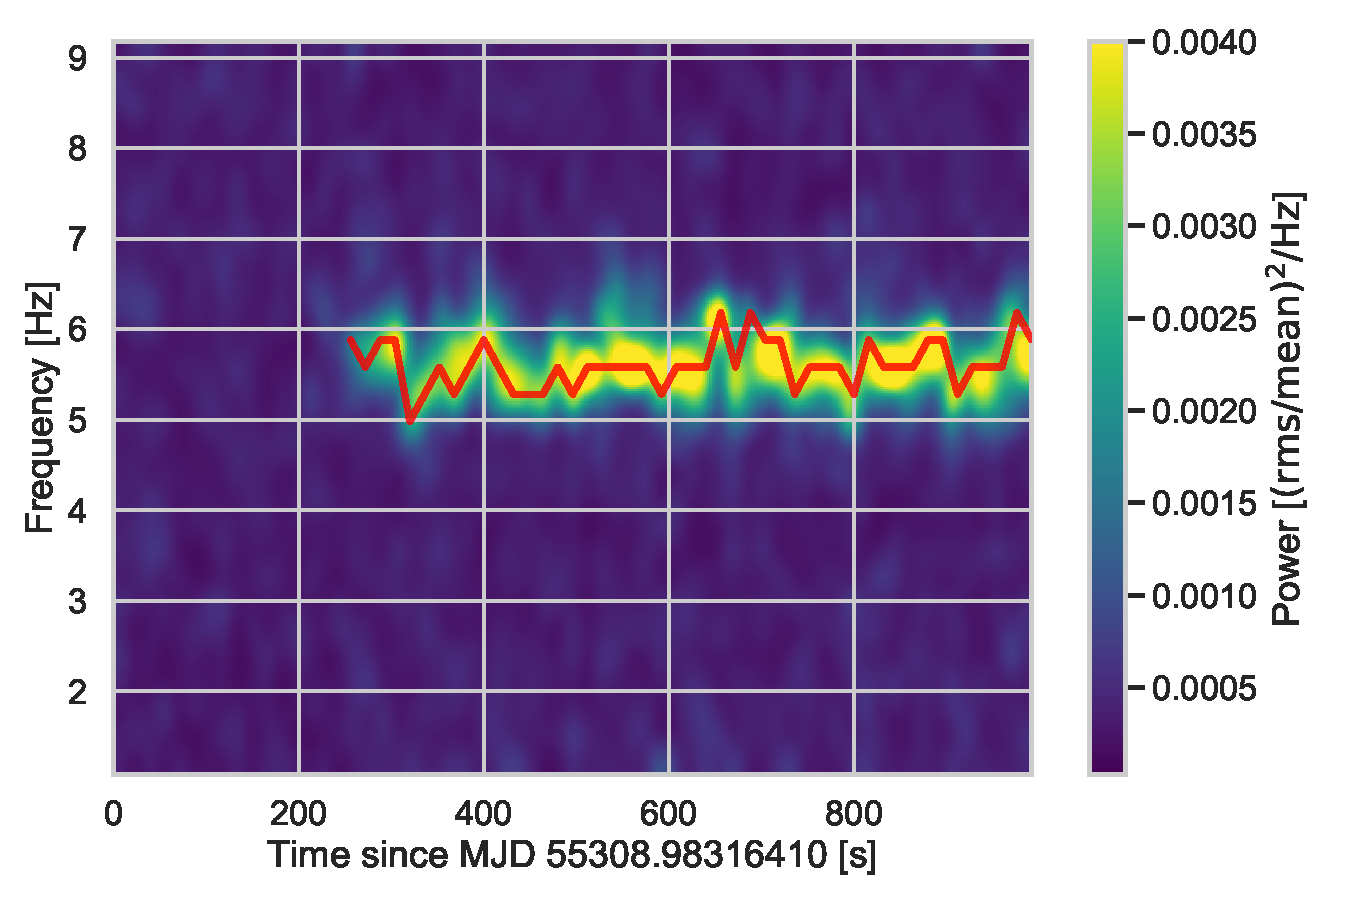
\includegraphics[width=9cm]{../figures/dyn_spec.pdf}
\caption{An example of a dynamic power spectrum generated from the GX-339 light curve shown in Figure \ref{fig:psd}. We generated 63 light curve segments of 16 seconds length with a $0.02\,\mathrm{s}$ time resolution and Fourier-transformed each to generate a power spectrum. The dynamic power spectrum here plots each power spectrum as a vertical slice as a function of time, with the colour indicating the fractional rms-normalized power in each bin (yellow are large powers, purple small) . The dynamic power spectrum was clipped to exclude the lowest and highest frequencies, and smoothed using bicubic interpolation to improve clarity. The QPO is clearly visible as a yellow streak, but seems not to be present during the entire observation. In red, we show the frequency with the highest power found in each segment (excluding frequencies below $3\,\mathrm{Hz}$ to exclude the low-frequency red noise), using the \mintinline{python}{trace_maximum} method.}
\label{fig:dynspec}
\end{center}
\end{figure}

For long observations with quasi-periodic oscillations (QPOs) spectrograms, more commonly known in the astronomy literature as Dynamic Power Spectra [REF], can be a useful way to track changes in the QPO centroid frequency over time. We have implemented \mintinline{python}{DynamicalPowerspectrum} as a subclass to \mintinline{python}{AveragedPowerspectrum} to provide this functionality. Like \mintinline{python}{AveragedPowerspectrum}, this class takes a \lightcurve object and a segment size as input, but instead of averaging the power spectra of each individual segment, it will create a matrix of time bins (one bin for each segment) as rows and Fourier frequencies as columns. Rebinning both along the time and frequency axis is possible. Moreover, the method \mintinline{python}{trace_maximum} automatically finds the frequency with the highest power in each segment in a given range of frequencies, and traces this maximum over time. An example using simulated data is shown in Figure \ref{fig:dynspec}.

Closely related to the cross spectrum and power spectrum are the crosscorrelation and the autocorrelation, implemented in classes \mintinline{python}{CrossCorrelation} and \mintinline{python}{AutoCorrelation}. As their respective Fourier spectra equivalents they take either one (autocorrelation) or two (cross correlation) \lightcurve objects as input and computes the correlation between the two light curves or of the single light curve with itself, along with the time lags for which the correlation was produced and the time lag at which the maximum correlation is measured.

It is useful to note that all classes in this section are compatible with Good Time Intervals. The classes \powerspectrum and \crossspectrum will generate warnings if the observations contain gaps; their averaged versions will take GTIs correctly into account by producing power spectra only from light curve segments for which data is available. 

%\noindent Here, $i = \sqrt{-1}$, and $A_{xj}, A_{yj}$ and $B_{xj}, B_{yj}$ describe the real and imaginary parts of the Fourier amplitudes, respectively . We restrict $\mathcal{F}_x(j)$ and $\mathcal{F}_y(j)$ to frequencies between $\nu_{j=0} = 1/T$ and the Nyquist frequency $\nu_{j=N/2} = 1/(2\Delta t)$.
%The complex cross spectrum is then calculated by multiplying the Fourier transform of light curve $\mathbf{x}$ with the complex conjugate of the Fourier transform of light curve $\mathbf{y}$ (, see also \citealt{uttley2014} for a recent review of spectral timing techniques):


%\subsection{Higher-Order Fourier Products and Spectral Timing Functionality}
%\label{sec:fourier_others}

%Over the past decade, higher-order Fourier products and spectral timing have emerged as key methods to study variability on different time scales as well as a function of wavelength. In \stingray, we have implemented several of the most common techniques, with plans to add to the existing tools as they become available in the future. Below, we will only give a brief description of each of the algorithms currently implemented in \stingray, with appropriate references where applicable.


%\subsubsection{Bispectrum and Biphase}



%* bispectrum/biphase

%\subsubsection{Covariance spectra}
%* Covariancespectrum/ AveragedCovarianceSpectrum

%%% FUTURE STUFF
%* RMSEnergySpectrum?
%* LagEnergySpectrum?
%* ExcessVarianceSpectrum?
 

%%% MODELLING FUNCTIONALITY %%%%%%%%%%%%%%%%%%%%%%%%%%%%%%%%%%%%%%%%%%%%%%%%%%%%%%%%%%%%%%%%%%%%%%%%%%%%%%%%%%%%%%

\section{The \texttt{modeling} Subpackage}
\label{sec:modeling}

Modelling data sets with parametric (often physically motivated) models that map an independent variable (e.g.\ time or frequency) to one or more dependent variables (e.g.\ flux, counts or Fourier powers) is a common task in astronomy. Constructing a general-purpose modelling framework is a highly non-trivial task, and better packages exist for general-purpose model building (e.g. STAN, \citealt{stan}), thus \stingray's modelling interface restricts itself to models of commonly used spectral-timing products, in particular modelling (averaged) power spectra. 
While it makes heavy use of the \verb|astropy.modeling.FittableModel| definitions, it uses custom definitions for fitting algorithms motivated by the statistical properties of spectral timing products, which deviate significantly from other data types commonly found in astronomy and thus cannot easily be modelled with standard approaches defined in \texttt{astropy}.

\subsection{General Overview}
The modelling subpackage logically separates out statistical models -- likelihoods and posteriors -- from the fitting functionality, such that different likelihoods and posteriors can be straightforwardly dropped in and out depending on the data set and problem at hand\footnote{This paper is not intended as an introduction into parametric modelling and statistical inference. For suitable introductions, we recommend e.g.~ \citet{hogg2010}}. In line with the overall philosophy of \stingray, the modelling subpackage is designed to be modular and easily extensible to specific problems a user might try to solve, while many typical tasks one might do with Fourier products are already built-in. It integrates with parts of the \verb|astropy.modeling| interface, and makes use of the \verb|scipy.optimize| interface for optimization as well as the package \texttt{emcee} for Markov Chain Monte Carlo (MCMC) sampling.

\subsection{Statistical Models}

All statistical models are implemented as a subclass of an Abstract Base Class \likelihood in module \verb|stingray.posterior|. In its most basic form, each subclass of \likelihood takes data in some form (most commonly two arrays, one with the independent and one with the dependent variable) as well as an object of type \verb|astropy.modeling.FittableModel|. The likelihood itself is implemented in the \texttt{evaluate} method, which takes a set of parameters to be passed to the \verb|astropy.modeling.FittableModel| instance, computes model values for each data point in the array of independent variables and statistically compares these model values with the data points stored in the dependent variable, assuming the particular statistical distribution of the likelihood definition. The result is a single quantity, which can then be e.g.~ optimized in order to find a Maximum Likelihood (ML) solution.

For all \likelihood subclasses implemented in \stingray, there will also be an appropriate subclass of \verb|stingray.modeling.Posterior| available. As with the \likelihood subclasses, subclasses of class \verb|Posterior| take data of some form and an \verb|astropy.modeling.FittableModel| instance upon instantiation. Additionally, all subclasses of  \verb|Posterior| also require definition of a \texttt{logprior} method, which calculates the value of the prior distributions on the parameters given a particular set of parameters. Because priors are strongly problem-dependent, they cannot be hard-coded into stingray. Even for relatively straightforward problems such as modelling quasi-periodic oscillations of X-ray binaries, the physical properties and their effect on the data can differ strongly from source to source, indicating that a prior set for Cygnus X-1 may not be appropriate for e.g.~ GRS 1915+105. Separating out the likelihood and posterior in distinct classes makes it possible to allow the use of the likelihood for maximum likelihood estimation, while requiring priors for estimating the Bayesian posterior probability through e.g.~ Markov Chain Monte Carlo simulations.

%There are two ways to define priors: they can be passed into the \texttt{priors} keyword argument upon instantiation of the class, or they can be set using the \verb|set_logprior| utility function in \verb|stingray.modeling|. In either case, the priors should be passed as a dictionary of \verb|"parameter name": distribution| pairs, where the parameter names match those of the \verb|astropy.modeling.FittableModel| instantiated and each distribution is a function definition that takes a parameter value and returns the probability density at that parameter value. \verb|stingray.modeling.Posterior| subclasses generally have three outward-facing methods: \verb|Posterior.logprior|, \verb|Posterior.loglikelihood| and \verb|Posterior.logposterior|. All three take a list of parameters as input. In addition, a \verb|__call__| method that executes \verb|logposterior| will allow the user to call the class instance directly and compute the log-posterior of the model given a set of input parameters. 

\texttt{Loglikelihood} and \texttt{Posterior} subclass definitions currently exist within \stingray for a range of different statistical models useful in the context of astronomical data. 
\verb|GaussianLogLikelihood| and \texttt{GaussianPosterior} implement statistical models for data with normally distributed uncertainties. \texttt{GaussianLogLikelihood} will compute what astronomers generally call $\chi^2$, because the likelihood calculated by this statistical model generally follows a $\chi^2$ distribution with $N-P$ degrees of freedom (where $N$ is the number of data points and $P$ the number of free parameters). Note, however, that this is \textbf{not} the same as the $\chi^2$ likelihood defined below!

\texttt{PoissonLogLikelihood} and \texttt{PoissonPosterior} calculate the likelihood and posterior for Poisson-distributed data, respectively. This likelihood is equivalent to what in astronomy is often called the \textit{Cash statistic} \citep{cash1979} and is the appropriate likelihood to use for count- or event-type data often found in X-ray astronomy time series and spectra.

\texttt{PSDLogLikelihood} and \texttt{PSDPosterior} implement the statistical model appropriate for modelling (averaged) power spectra, a $\chi^2$ distribution. We broke with the rule of naming likelihoods and posteriors after the statistical distribution they implement in this case, because as mentioned above, astronomers tend to call the likelihood for normally distributed data $\chi^2$, and this naming helps avoid any confusion. These two classes implement a $\chi^2_2$ distribution for Fourier spectra generated with the \powerspectrum class, and a $\chi^2_{2MK}$ distribution for power spectra generated with the \texttt{AveragedPowerspectrum} class, where $M$ is the number of averaged segments and $K$ is the number of averaged neighbouring frequency bins. Please note that as laid out in \citet{huppenkothen2017}, these distribution are \textbf{not} appropriate for use on (averaged) cross spectra. The appropriate distributions for these products will be implemented in a future version of \stingray.

Other statistical models can be easily implemented by subclassing the \texttt{LogLikelihood} and \texttt{Posterior} Abstract Base Classes and using the existing classes as template.

\begin{figure*}[htbp]
\begin{center}
%\begin{subfigure}[b]{11.0cm}
\subfloat[plot]{%
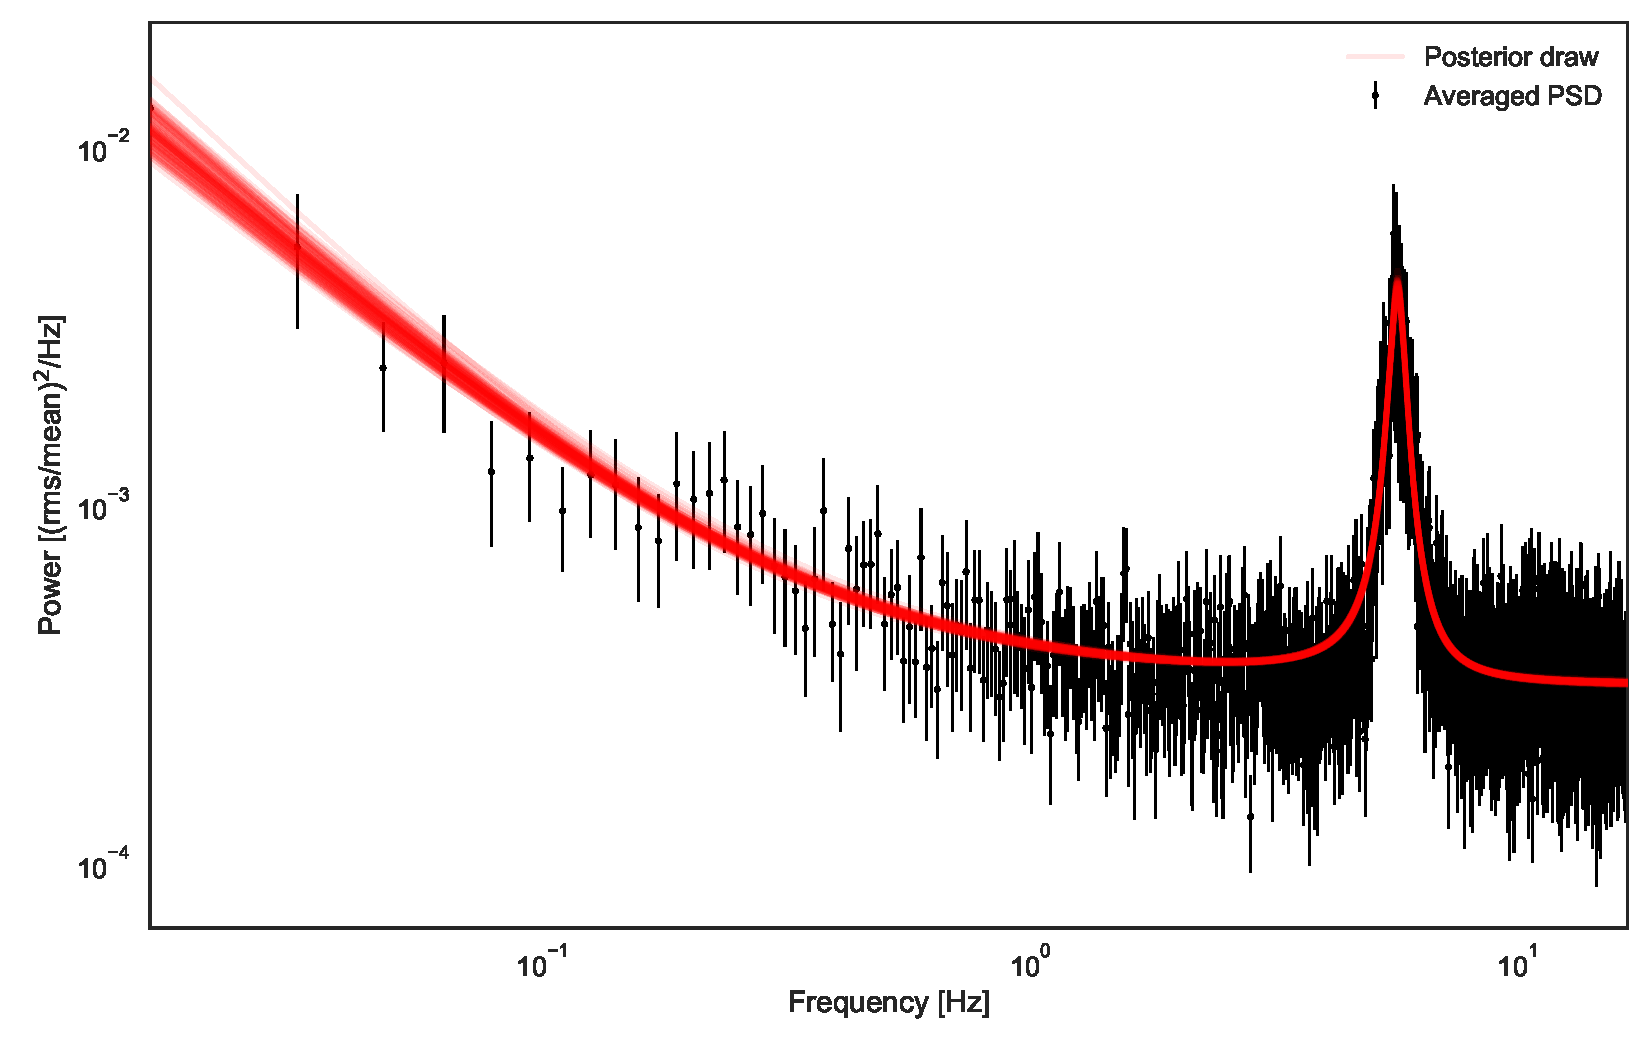
\includegraphics[width=10cm]{../figures/example_posterior.pdf}
}%\end{subfigure}
%\begin{subfigure}[b]{6.8cm}
\subfloat[plot]{%
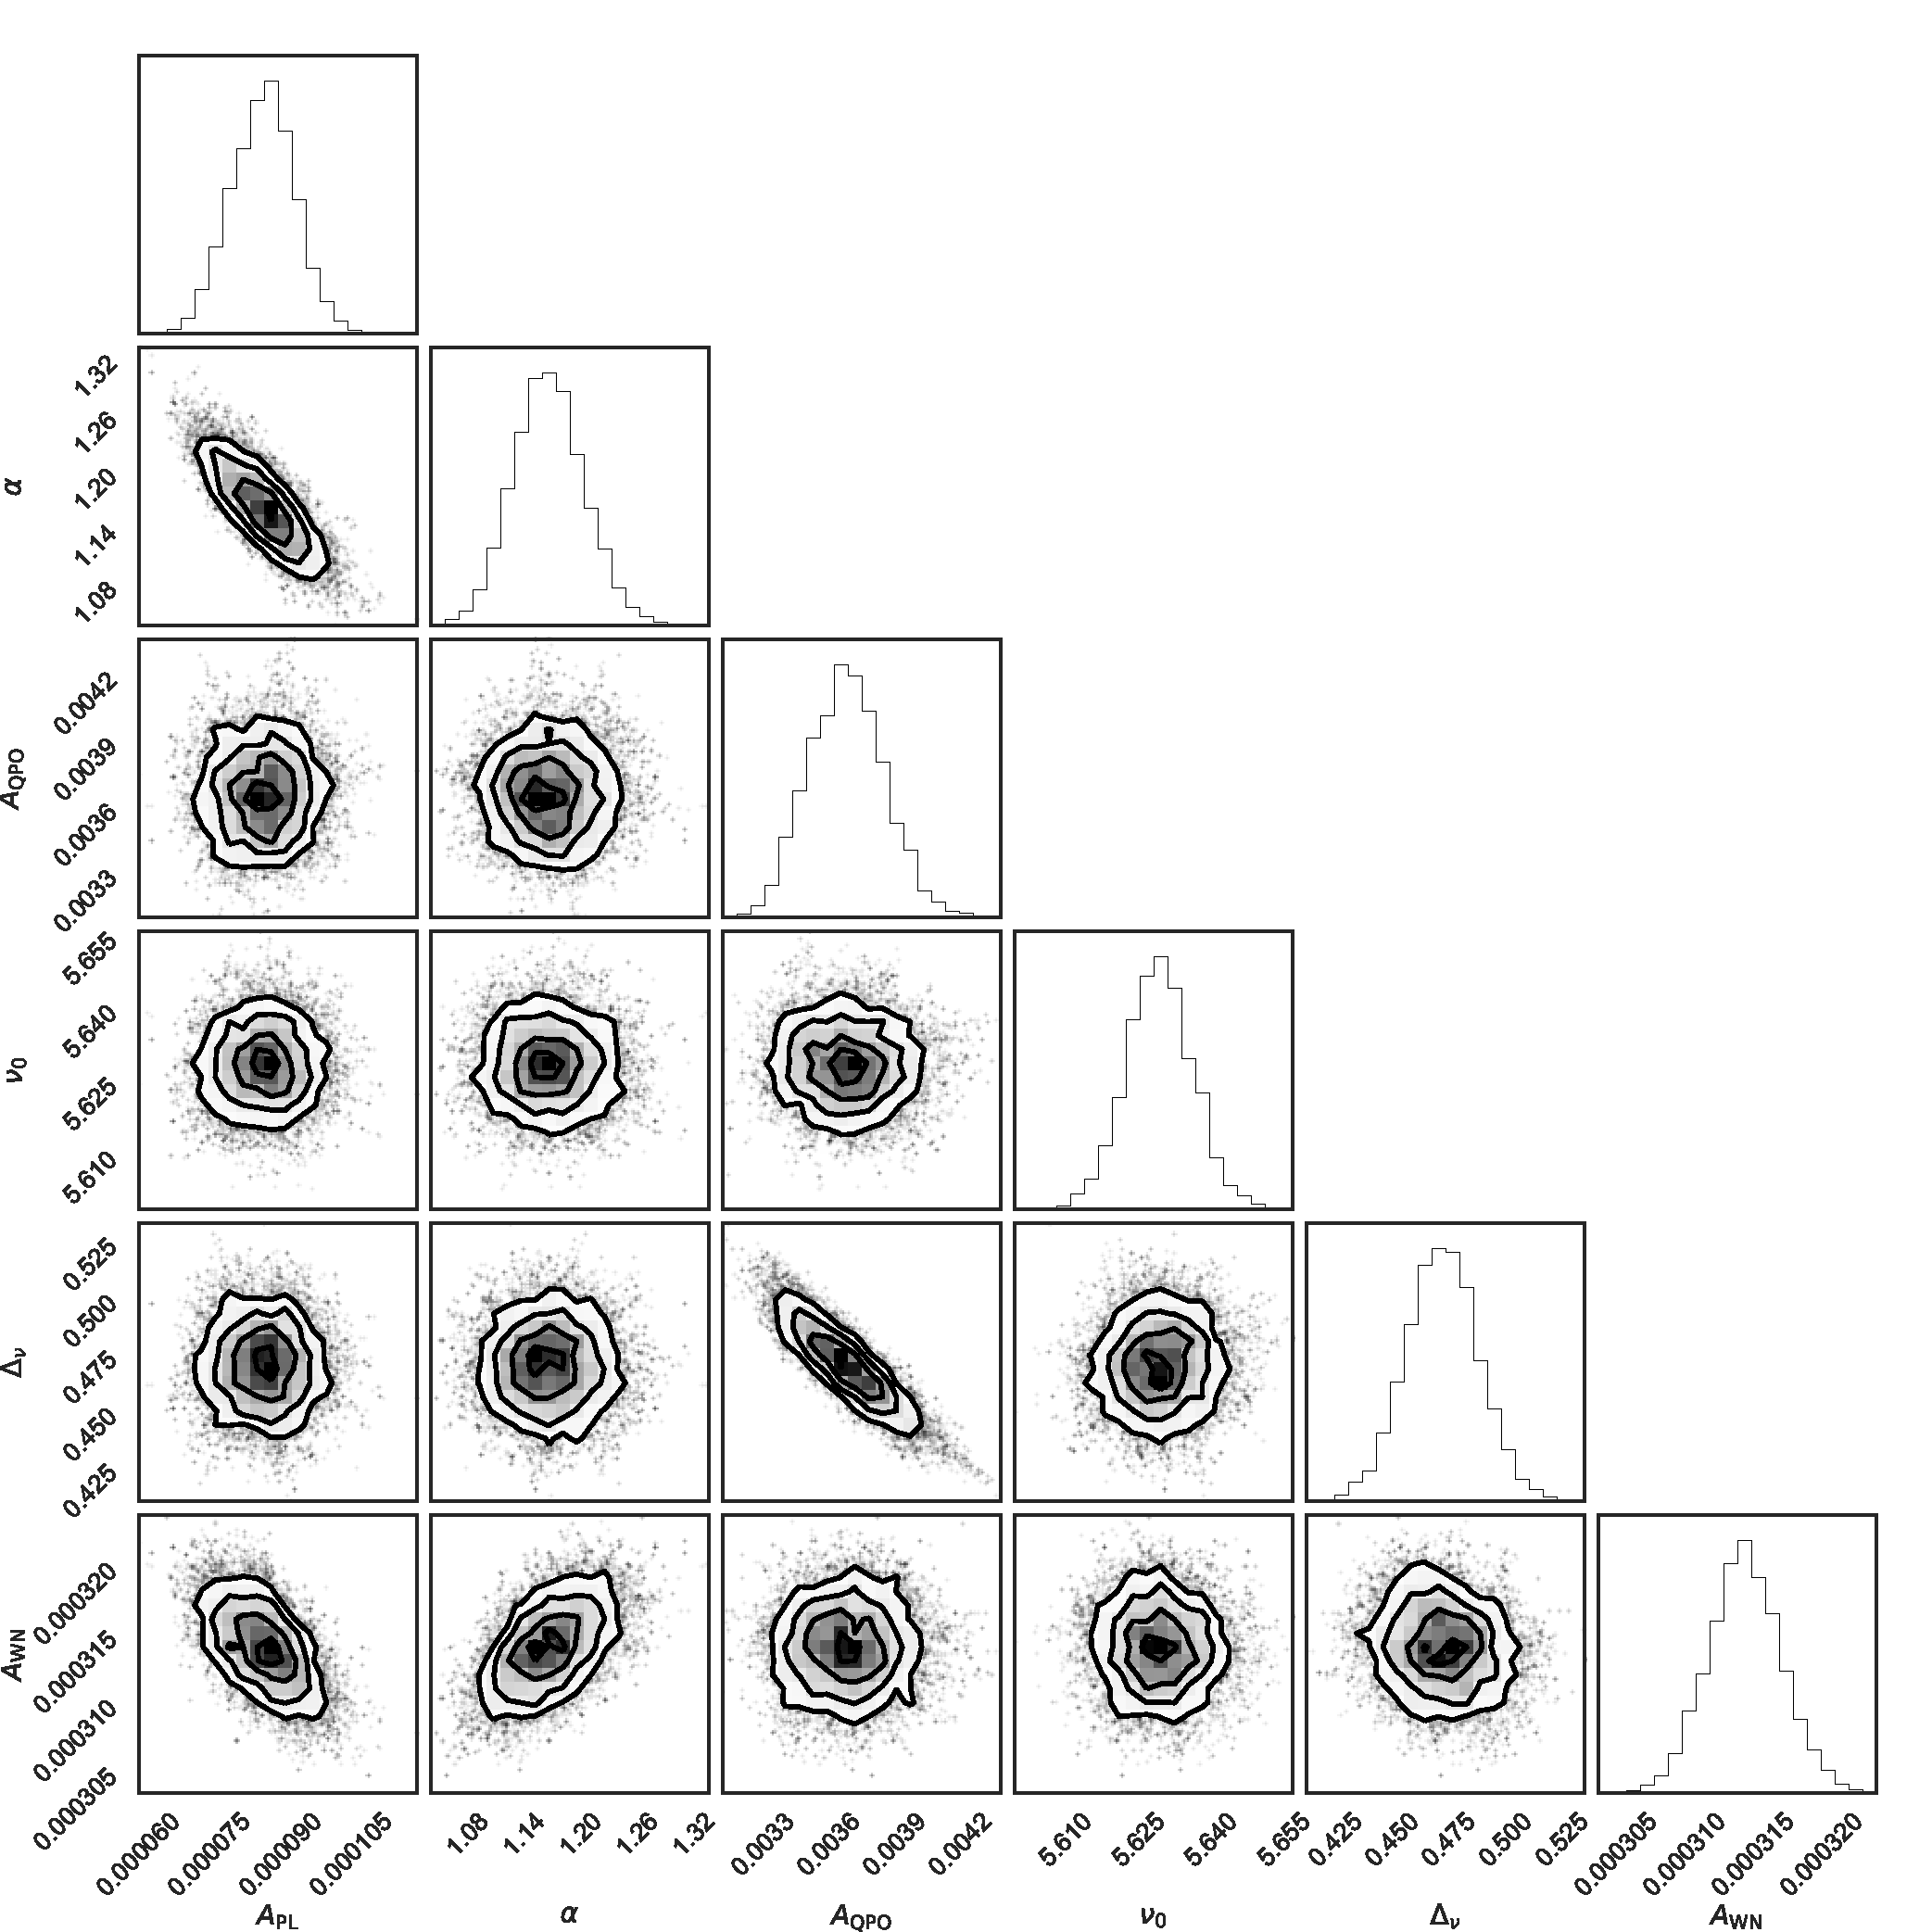
\includegraphics[width=6.5cm]{../figures/example_psd_corner.pdf}
}%\end{subfigure}
\caption{Left panel: In black, a power spectrum averaged out of 15 light curve segments of 64s each of the GX 339-4 observation, along with draws from the posterior distribution of the power law model plus the Lorentzian QPO model and constant used to represent the data (red). Right panel: corner plot showing the marginal posterior distributions (diagonal) of the six parameters of the model: the amplitude of the power law $A_\mathrm{PL}$, the power law index $\alpha$, the amplitude of the Lorentzian $A_\mathrm{QPO}$, the QPO centroid frequency $\nu_0$, the width of the QPO $\Delta_\nu$, and the amplitude of the white noise, $A_\mathrm{WN}$. The right-hand figure was produced using the package \texttt{corner} \citep{corner}.}
\label{fig:posterior}
\end{center}
\end{figure*}

\subsection{General Parameter Estimation and Model Comparison Functionality}

Stingray implements utility functions in order to reduce some of the overhead required for standard parameter estimation and model comparison tasks. Im particular, the \verb|parameterestimation| module implements a range of classes and functions to aid users in fitting models to data and estimating the probability distributions of parameters.

The class \texttt{ParameterEstimation} provides the basis for more sophisticated, specialized implementations for particular data types. Its core methods are \verb|fit| and \verb|sample|. The former takes an instance of a \verb|LogLikelihood| or \verb|Posterior| subclass and uses minimization algorithms implemented in \verb|scipy.optimize| to find the Maximum Likelihood (ML) or Maximum-A-Posteriori (MAP) solution. The \verb|sample| method uses the Affine-Invariant MCMC sampler implemented in \texttt{emcee} \citep{emcee} to generate samples from a posterior distribution passed as an instance of a subclass of \verb|Posterior|. Note that \textit{you should never pass a} \verb|LogLikelihood| \textit{instance into the} \verb|sample| \textit{method}, because sampling from a likelihood is statistically invalid. In addition to these core methods, higher-level functionality implemented in this class includes calculating the Likelihood Ratio Test (LRT) for two different models $M_1$ and $M_2$ via the \verb|compute_lrt| method (note the statistical assumptions of the LRT, and where they fail, e.g. \citealt{protassov2002}). In addition, the \verb|calibrate_lrt| method allows calibrating the p-value for rejecting the model $M_1$ via simulations of $M_1$, using either an MCMC sample (for Bayesian inference) or the covariance matrix derived from the optimization (both Bayesian and Maximum Likelihood approaches).

Stingray also implements two classes that summarize results of the optimization and sampling procedures in concise, useful ways. The \verb|fit| method returns an instance of class \verb|OptimizationResults|. This contains the most important outputs from the optimizer, but will also behind the scenes calculate a number of useful quantities, including the covariance between parameters (or a numerical approximation for some minimization algorithms), the Akaike and Bayesian Information Criteria (AIC: \citealt{akaike1974}; BIC: \citealt{schwarz1978}) as well as various summary statistics.%, e.g. the figure of merit, defined as 

%\[
%m = \sum_{j=1}^{N}{\left( \frac{y_j - \nu_j}{\nu_j} \right)^2} \,
%\]
%\noindent where $\mathbf{D} = \{x_j, y_j\}_{j=1}^{N}$ is the set of $N$ data points and $\nu_j$ is the value of the model evaluated at each $x_j$.

Similarly, an instance of class \verb|SamplingResults| is returned by the \verb|sample| method, which returns the posterior samples calculated by the MCMC sampler, as well as computes a number of helpful quantities using the MCMC chains. It calculates useful diagnostics including the acceptance fraction, the autocorrelation length and the Rubin-Gelman statistic \citep{gelman1992} to indicate convergence, and infers means, standard deviations and user-defined credible intervals for each parameter.

%Both \verb|OptimizationResults| and \verb|SamplingResults| implement a \verb|print_results| and a \verb|plot_results| method, which produce useful text output for log files and diagnostic plots that help understand the results.

\subsection{Special Functionality for Fourier Products}

The subclass \verb|PSDParEst| inherits directly from \verb|ParameterEstimation| and implements a number of additional methods particularly useful for modelling power spectra. One particularly common task is to search for periodic signals (e.g. from pulsars) in a power spectrum, which reduces to finding outliers around an assumed power spectral shape (assuming the signal is \textit{strictly} periodic, and thus all power approximately concentrated in one bin). In the presence of other variability, the probability of observing a certain power $P_j$ at a frequency $\nu_j$ under the assumption that no periodic signal is present depends on the shape and parameters of the underlying power spectral model assumed to have generated the data. As \citet{vaughan2010} show, there is an inherent uncertainty in our inference of the parameters of this power spectral model, which must be taken into account via simulations. \verb|PSDParEst| implements a method \verb|calibrate_highest_outlier|, which finds the $k$ highest outliers (where $k$ is a user-defined number) and calculates the posterior predictive $p$-value that said outlier cannot be explained by noise alone. It makes heavy use of the method \verb|simulate_highest_outlier|, which uses the \verb|sample| method to derive an MCMC sample and then simulate fake power spectra from that model for a range of plausible parameter values in order to include our model uncertainty into the $p$-value. For details of the overall procedure, see \citet{vaughan2010}. 

As of this version, the \verb|stingray.modeling| subpackage has no functionality to model higher-order Fourier products. For spectral timing in particular, this would involve being able to read and apply instrument responses to models, as well as being able to interface with the library of spectral models associated with the X-ray spectral fitting tool XSPEC \citep{arnaud1996}. Providing this functionality is planned for a future release of \stingray. 

%For an example workflow describing how to model a power spectrum using \stingray, see the code example in the Appendix.


%%% SIMULATOR %%%%%%%%%%%%%%%%%%%%%%%%%%%%%%%%%%%%%%%%%%%%%%%%%%%%%%%%%%%%%%%%%%%%%%%%%%%%%%%%%%%%%%%%
\begin{figure*}[htbp]
\begin{center}
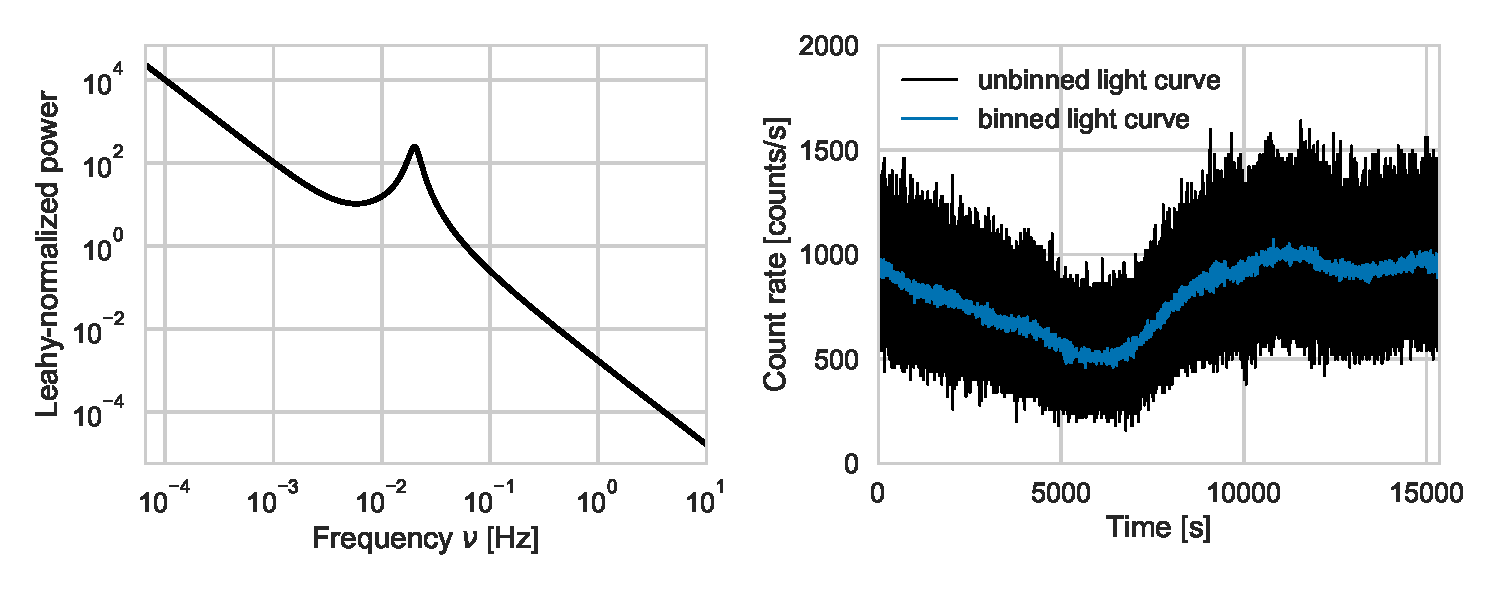
\includegraphics[width=\linewidth]{../figures/sim_lc.pdf}
\caption{Left: A power spectral shape generated using a compound `astropy.modeling.models` object of a power law and a Lorentzian. Right: A corresponding light curve generated by the \texttt{simulator} subpackage with a time resolution of $0.05\,\mathrm{s}$, a total duration of $15\,\mathrm{ks}$, a mean count rate of $40\,\mathrm{counts}/\mathrm{s}$ and a fractional rms amplitude of $0.2$. In blue we show a binned version of the same light curve.}
\label{fig:sim_lc}
\end{center}
\end{figure*}

\section{The \texttt{simulator} Subpackage}
\label{sec:simulator}

The \texttt{simulator} subpackage is designed as a flexible and quick way to generate simulated light curves out of known power spectral shapes. It uses the algorithm from \citet{timmer1995} to generate light curves out of a large range of different power spectral shapes, assuming a random assignment of (Gaussian-distributed) phases of the Fourier amplitudes. 
It is capable of generating light curves in different (given) energy bins, using impulse response functions in order to mimic behaviour observed from real sources. It can take both \texttt{astropy.modeling.models} objects as well as a user-given array of powers, and optional an array specifying the impulse response function in the case of generating multiple light curves in different energy bins.

In Figure \ref{fig:sim_lc}, we present a light curve as generated by a given power spectral shape. The output is a \texttt{Lightcurve} object that can be used like real data sets, including all functionality related to GTIs, spectral-timing products and modelling. 

[\textbf{MATTEO:} Do you have any functionality you'd like to expand on in here?]

%%% PULSAR FUNCTIONALITY %%%%%%%%%%%%%%%%%%%%%%%%%%%%%%%%%%%%%%%%%%%%%%%%%%%%%%%%%%%%%%%%%%%%%%%%%%%%%%%%%%%%%%%%

\section{The \texttt{pulse} Subpackage}
\label{sec:pulsar}
The \stingray subpackages \texttt{pulse} contains the basic operations to perform the search and characterization of pulsed signals for use e.g.\ in searches of X-ray pulsars.

\subsection{Epoch Folding}
Among the basic algorithms used in pulsar astronomy, one cannot overstate the importance of Epoch Folding (EF).
The algorithm consists of cutting the signal at every pulse period and summing all sub-intervals in phase. 
An alternative way of seeing it, more useful for photon data, is as a \textit {histogram of pulse phases}.

If the period is exactly correct and assuming a stable pulsation, the signal-to-noise ratio will get better approximately with the square root of the number of summed sub-intervals [REF].
This is the method used to obtain practically all pulse profiles shown in the literature, as most pulsar signals are orders of magnitude below noise level.

The \texttt{pulse.pulsar} submodule contains the functionality to calculate the phase given a simple pulse ephemeris consisting of any number of pulse frequency derivatives%
\footnote{For more complicated cases, like binary pulsars or long-term pulsar noise not well described by pulse derivatives, we recommend to look at more focused libraries like \href{https://github.com/nanograv/PINT}{PINT} [REF]}.
Moreover, the module also includes a mechanism to calculate the exposure of single bins in the pulse profile. 
This is particularly useful for very long-period pulsars where the pulsed period is comparable to the length of the GTIs.
The different exposure of pulse bins caused by the absence of signals during GTIs is taken into account in the calculation of the final pulse profile by the folding algorithm, if the user asks for it. 

\subsection{Epoch Folding Searches and \zsq Searches}
\label{sec:efzsq}
During a search for pulsations, the first step is usually the PDS. 
However, often pulsations do not leave a clear signature above noise level in the PDS, because they are weak or they fall close to bin edges, where the sensitivity is reduced [REF].
Even when they do, the frequency resolution of the PDS is often inadequate to measure precisely the pulse frequency.
Therefore, an additional statistical analysis is needed. 

The Epoch Folding Search (EFS) method consists of executing the folding at many trial frequencies around the candidate frequency.
Once the folding is performed, the following statistics is calculated on the profile:
\begin{equation}
\mathcal{S} = \sum_i\frac{(P_i - \overline{P})^2}{\sigma^2}
\end{equation}
where $P_i$ are the bins of the profile, $\overline{P}$ is the mean level of the profile, and $\sigma$ is the standard deviation.
$\mathcal{S}$ is the summed squared error of the actual pulsed profile with respect to a \textit{flat} model, and follows a $\chi^2$ distribution.

If there is no pulsation, $\mathcal{S}$ will assume a random value distributed around the number of degrees of freedom $n - 1$ (where $n$ is the number of bins in the profile) with a well defined statistical distribution ($\chi^2_{n - 1}$) that allows an easy calculation of detection limits. 
When observing a peak of given height is very unlikely under the null hypothesis (meaning that the probability to obtained this peak by noise is below a certain $\epsilon$), this peak is considered a pulse candidate.
If the frequency resolution is sufficiently high, close to the correct frequency, as described by \citep{leahy1983b,leahy1987}, the peak in the epoch folding periodogram has the shape of a $\mathrm{sinc}^2$ function whose width is driven by the length of the observation.

The epoch folding statistics, however, can give the same value for a pulse profile at the correct frequency and, for example, an harmonic that produces a deviation from a Poisson distribution.
A more effective method is the $Z^2_n$ statistics \citep{buccheri1983}, which is conceptually similar to EF but has high values when the signal is well described by a small number of sinusoidal harmonics: 

\begin{equation}
\zsq = \dfrac{2}{N} \sum_{k=1}^n \left[{\left(\sum_{j=1}^N \cos k \phi_j\right)}^2 + {\left(\sum_{j=1}^N \sin k \phi_j\right)}^2\right] \; ,
\end{equation}

\noindent where $N$ is the number of photons, $n$ is the number of harmonics, $\phi_j$ are the phases corresponding to the event arrival times $t_j$ ($\phi_j = \nu t_j$, where $\nu$ is the pulse frequency).

The \zsq statistics defined in this way, far from the pulsed profile, follows a $\chi^2_n$ distribution, where $n$ is the number of harmonics this time.
This allows, again, to easily calculate thresholds based on the probability of obtaining a given \zsq by pure noise.

The standard \zsq search calculates the phase of each photon and calculates the sinusoidal functions above for each photon.
This is very computationally expensive if the number of photons is high. 
Therefore, in Stingray, the search is performed by binning the pulse profile first and using the phases of the folded profile in the formula above, multiplying the squared sinusoids of the phases of the pulse profile by a weight corresponding to the number of photons at each phase.

\begin{equation}
\zsq \approx \dfrac{2}{\sum_j{w_j}} \sum_{k=1}^n \left[{\left(\sum_{j=1}^m w_j \cos k \phi_j\right)}^2 + {\left(\sum_{j=1}^m w_j \sin k \phi_j\right)}^2\right]
\end{equation}

Since the sinusoids are only executed on a small number of bins, while the epoch folding procedure just consists of a very fast histogram-like operation, the speedup of this new formula is obvious. 
Care must be put into the choice of the number of bins, in order to maintain a good approximation even when the number of harmonics is high. 
We recommend in the documentation to use a number of bins at least 10 times larger than the number of harmonics.

\subsection{Characterization of pulsar behavior}
\label{sec:ephem}
As seen in Section~\ref{sec:efzsq}, the \zsq or the EF periodograms of a perfectly stable pulsation have the shape of a $\mathrm{sinc}^2$ function.
\stingray has functionality to fit these periodograms with a $\mathrm{sinc}^2$ funtion or alternatively a Gaussian model, and find the mean frequency with high precision.

A significant deviation from the expected shape from these models can happen if the pulsation is not stable.
Calculating the \textit{periodogram} is an option to investigate how the pulse phase varies in time.
The periodogram in this context consists of a 2D histogram of the phase and arrival times of the pulses. 
If the pulsation is stable and the pulse frequency was determined with precision, the periodogram shows vertical stripes corresponding to perfectly aligned pulses.
If the frequency is not as precise, the stripes become more and more diagonal.
If the pulse has a detectable frequency derivative, these stripes bend with a parabolic shape.

A very precise way to determine the exact pulse ephemeris is out of the scope of \stingray. 
However, \stingray has a mechanism to calculate the pulse arrival times (or times of arrival, TOAs) using a pulse template, using the \texttt{fftfit} algorithm used for radio pulsars. 
This is implemented in the \texttt{get\_TOA} function in \texttt{stingray.pulse.pulsar}.
Then, the user can use the TOAs with more specialized software like Tempo, Tempo2 or PINT.

[Fig. XXXX: a variation of the pulse phase corresponding to a period derivative. ]
[\textbf{MATTEO}: you put this here for a figure. Do you have a handy way to make one?!]


%%% DEVELOPMENT + INTEGRATION %%%%%%%%%%%%%%%%%%%%%%%%%%%%%%%%%%%%%%%%%%%%%%%%%%%%%%%%%%%%%%%%%%%%%%%%%%%%%%%%%%

\section{Development and Integration Environment}
\label{sec:development}

\stingray is developed entirely in Python3, with backwards compatibility to Python 2.7 where possible through the integration package \texttt{six}. Development is version-controlled through \texttt{git}, and officially hosted through an organization on \textit{GitHub}, where several interconnected repositories related to \stingray live, including the core library, extension packages \hendrics and \texttt{DAVE}, as well as the suite of tutorials and this manuscript. All patches and code are submitted via pull requests to the \stingray repository, and checked by a maintainer for correctness and adherence to standards of code, documentation and tests. As an \textit{Astropy} Affiliated Package\footnote{\url{http://www.astropy.org/affiliated/}}, we follow the coding standards as well as community guidelines (including the Code of Conduct) set out by the \textit{Astropy} community. 
All code within the \stingray core library is subject to extensive unit testing, with compatibility across platforms as well as different versions of Python and required packages controlled through Continuous Integration services \textit{Travis} (Unix platforms) and \textit{AppVeyor} (Windows). Test coverage is checked using \textit{Coveralls}. 
All user-facing functions and classes within \stingray must have documentation in the form of docstrings, compiled and built along with the main documentation pages using \textit{sphinx} and hosted on \texttt{readthedocs}\footnote{\url{https://stingray.readthedocs.io/en/latest/}}. Tutorials are provided in the form of executable \textit{Jupyter} notebooks in a separate repository\footnote{\url{https://github.com/stingraySoftware/notebooks}}, which can either be run interactively using \textit{Binder} or viewed as part of the documentation. 


%%% HENDRICS + DAVE %%%%%%%%%%%%%%%%%%%%%%%%%%%%%%%%%%%%%%%%%%%%%%%%%%%%%%%%%%%%%%%%%%%%%%%%%%%%%%%%%%%%%%%%%
\section{\hendrics: A Command-Line Interface for \stingray}
\label{sec:hendrics}

The \hendrics package\footnote{\url{https://github.com/stingraySoftware/hendrics}}---formerly called \texttt{MaLTPyNT} \citep{bachetti2015b}---builds upon \stingray by providing a suite of easy-to-execute command-line scripts whose primary use is providing an accurate quick-look (spectral-)timing analysis of X-ray observations, useful for a range of use cases, including exploratory data analysis and quality assessment of larger data analysis pipelines. While its initial development proceeded independently from \stingray, much of its core functionality since version 3.0 is based on the classes and methods \stingray provides, and some key functionality has been shifted to \stingray where appropriate. 

Its key distinguishing feature from established command-line interfaces such as FTOOLS is the accurate treatment of gaps in the data (for example due to the Earth's occultation or the South Atlantic Anomaly), as well as its treatment of dead time for certain detectors like \nustar. Where \stingray aims to provide flexible building blocks for designing sophisticated spectral-timing analysis workflows, \hendrics provides end-to-end solution for common tasks such as power density and cross spectra, time lags, pulsar searches, colour-colour as well as colour-intensity diagrams, at the cost of loosing some flexibility during the creation of those products. Like \stingray, \hendrics is an \astropy affiliated package and aims to build upon and be compatible with functionality provided as part of the \astropy ecosystem.
\hendrics supports a range of output data formats including netCDF4 and ASCII formats, which can then be read into other astronomical data analysis systems such as XSPEC \citep{arnaud1996} or ISIS  \citep{houck2000}.

\hendrics is in release version 4 as of 2018-02-12, and under active development, utilizing the same continuous integration, testing and code review standards as \stingray.


\begin{figure*}[htbp]
\begin{center}
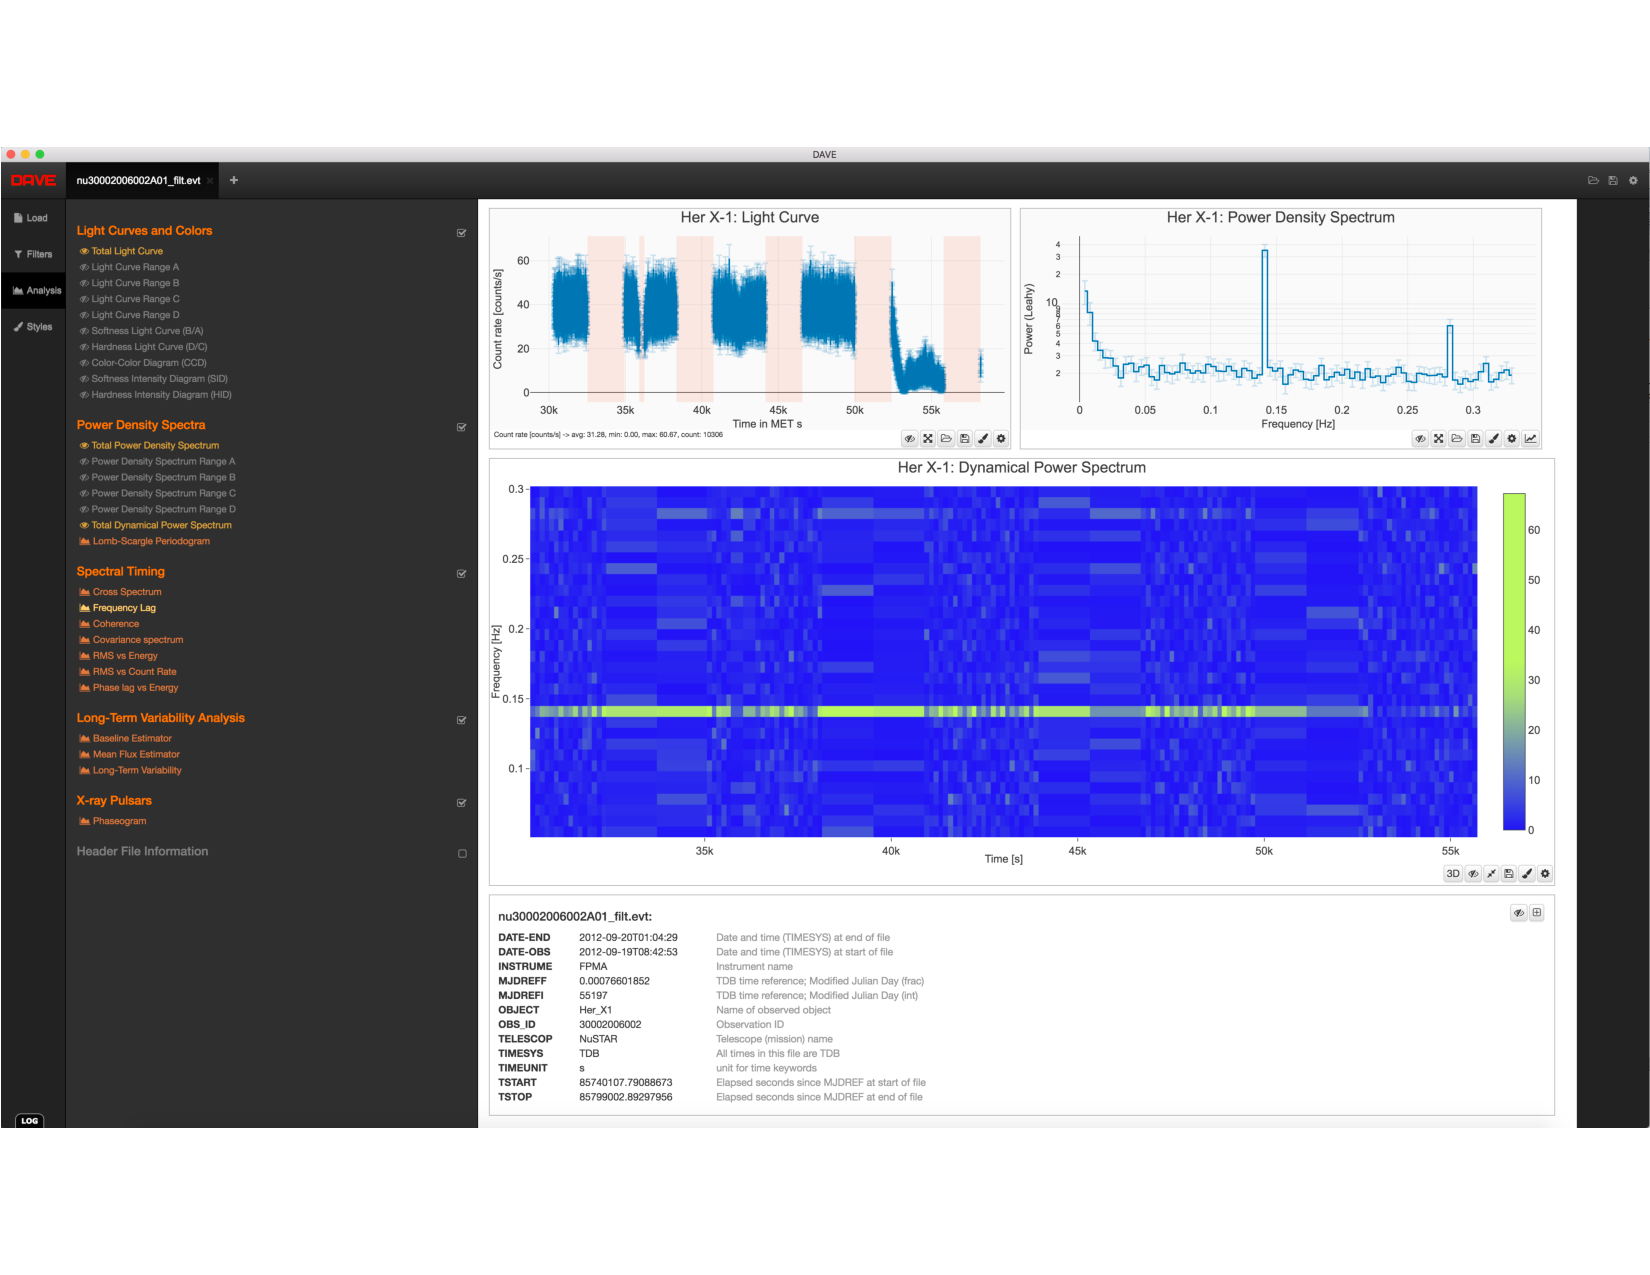
\includegraphics[width=\linewidth]{../figures/dave.pdf}
\caption{An example of the \dave graphical user interface for the Her X-1 pulsar data observed with \nustar: At the top left, the last 30ks of the pulsar light curve with the GTIs clearly marked. In the top right, the averaged power spectrum generated from 109 segments of $256\,\mathrm{s}$ duration with a binned time resolution of $1.5\,\mathrm{s}$. In the middle, we present the dynamic power spectrum generated from the same $256\,\mathrm{s}$ segments that generated the top right averaged power spectrum. Below, header meta-data is shown for reference. On the left, the menu presents a range of options of figures to plot and compare, including spectral-timing capabilities. All figures are interactive, including panning and zooming, as well as interactive choices of data selection.}
\label{fig:dave}
\end{center}
\end{figure*}

\section{\texttt{DAVE}: Exploratory Data Analysis in a Graphical User Interface}
\label{sec:dave}

\dave\footnote{\url{https://github.com/stingraySoftware/dave}}---the Data Analysis for Variable Events package---is a Graphical User Interface built on top of \stingray in order to provide users with interactive capabilities for exploratory data analysis on time series in general, and variable sources in particular. Its goal is to enable scientific exploration of astronomical X-ray observations in a graphical environment. Much of the core functionality within \stingray is available in \dave as well: creation of power spectra, cross spectra, dynamic power spectra and spectral-timing products such as time lags, coherence measurements. In addition, it implements interactive filtering of light curves with respect to energy channels or energies (if a response matrix file is loaded), time ranges, and count rates. Users may compare light curves and power spectra from different energy ranges, and may create auxiliary products such as colour-colour and colour-intensity diagrams that further aid the exploration of the data. An example of the interface is shown in Figure \ref{fig:dave}. The full interface and its capabilities will be described in a forthcoming publication. 


%%% FUTURE DEVELOPMENT %%%%%%%%%%%%%%%%%%%%%%%%%%%%%%%%%%%%%%%%%%%%%%%%%%%%%%%%%%%%%%%%%%%%%%%%%%%%%%%%%%%%%%%

\section{Future Development Plans}
\label{sec:future}

Future plans for \stingray development are largely aimed at extending current functionality related to Fourier spectra (with e.g.~ the planned implementation of the statistical distributions relevant to co-spectra; \citealt{huppenkothen2017}), and continuing work towards comprehensive spectra-timing capabilities. While reference implementations of higher-order Fourier products such as bispectra (bicoherence?) and biphase exist [do you want refs for these?], they require additional extensions to be useful to science. New key features in the next version of \stingray, based on an existing reference implementation of covariance spectra \citep{WilkinsonUttley09}, will include lag-energy spectra \citep{Vaughanetal94}, RMS-energy spectra \citep{Revnivtsevetal99}, and excess variance spectra \citep{Vaughanetal03}. In addition, while at the moment, there is rudimentary functionality to build spectra-timing products, it is currently not possible to seamlessly work with these products using \stingray, because \stingray currently has no native capability for energy-spectral modelling. Instead, they would have to be exported (e.g. saved to disk) and then loaded into another software, significantly disrupting workflows and pipeline development. In order to streamline this process, we aim to connect \stingray with existing packages for modelling X-ray spectra. Here, it will be necessary to connect \stingray with the extensive suite of physical models implemented in XSPEC, as well as existing spectral fitting codes implemented in \textit{Python}, most notably the open-source package \textit{Sherpa} \citep{sherpa}.

Data rates from current and future X-ray instruments are increasing at a precipitous rate, pushing memory and processing requirements for even simple tasks like Fast Fourier Transforms of data observed e.g.~ with \textit{NuSTAR} and \textit{AstroSAT} \citep{singh2014} into a regime that is difficult with standard desktop computing architectures. Therefore, the other strong emphasis for the second version of \stingray will be code and algorithm optimization. Where possible, we will replace existing implementations by high-performance equivalents that take advantage of recent developments in computing (such as GPU-enabled computations and multi-core batch processing), and optimize and streamline existing code to minimize computational overhead and memory usage of the classes and functions implemented within \stingray. 

%%% ACKNOWLEDGMENTS + REFERENCES %%%%%%%%%%%%%%%%%%%%%%%%%%%%%%%%%%%%%%%%%%%%%%%%%%%%%%%%%%%%%%%%%%%%%%%%%%%%%%%

%% If you wish to include an acknowledgments section in your paper,
%% separate it off from the body of the text using the \acknowledgments
%% command.
\acknowledgments
DH acknowledges support from the DIRAC Institute in the Department of Astronomy at the University of Washington. The DIRAC Institute is supported through generous gifts from the Charles and Lisa Simonyi Fund for Arts and Sciences, and the Washington Research Foundation.
We thank Astro Hack Week for providing the venue that started this project and the Lorentz Centre for organizing the workshop that started the collaboration. We thank the Google Summer of Code Program for funding a total 5 students who implemented a large fraction of the various library components over two summers.

%% To help institutions obtain information on the effectiveness of their 
%% telescopes the AAS Journals has created a group of keywords for telescope 
%% facilities.
%
%% Following the acknowledgments section, use the following syntax and the
%% \facility{} or \facilities{} macros to list the keywords of facilities used 
%% in the research for the paper.  Each keyword is check against the master 
%% list during copy editing.  Individual instruments can be provided in 
%% parentheses, after the keyword, but they are not verified.

%\vspace{5mm}
%\facilities{HST(STIS), Swift(XRT and UVOT), AAVSO, CTIO:1.3m,
%CTIO:1.5m,CXO}

%% Similar to \facility{}, there is the optional \software command to allow 
%% authors a place to specify which programs were used during the creation of 
%% the manusscript. Authors should list each code and include either a
%% citation or url to the code inside ()s when available.

%\software{astropy \citep{2013A&A...558A..33A},  
%          Cloudy \citep{2013RMxAA..49..137F}, 
%          SExtractor \citep{1996A&AS..117..393B}
%          }

%% Appendix material should be preceded with a single \appendix command.
%% There should be a \section command for each appendix. Mark appendix
%% subsections with the same markup you use in the main body of the paper.

%% Each Appendix (indicated with \section) will be lettered A, B, C, etc.
%% The equation counter will reset when it encounters the \appendix
%% command and will number appendix equations (A1), (A2), etc. The
%% Figure and Table counter will not reset.

%\appendix


\bibliography{stingraypaper}
\bibliographystyle{aasjournal}


%\begin{thebibliography}{}

%\bibitem[Astropy Collaboration et al.(2013)]{2013A&A...558A..33A} Astropy Collaboration, Robitaille, T.~P., Tollerud, E.~J., et al.\ 2013, \aap, 558, A33 
%\bibitem[Bertin \& Arnouts(1996)]{1996A&AS..117..393B} Bertin, E., \& Arnouts, S.\ 1996, \aaps, 117, 393 
%\bibitem[Corrales(2015)]{2015ApJ...805...23C} Corrales, L.\ 2015, \apj, 805, 23
%\bibitem[Ferland et al.(2013)]{2013RMxAA..49..137F} Ferland, G.~J., Porter, R.~L., van Hoof, P.~A.~M., et al.\ 2013, \rmxaa, 49, 137
%\bibitem[Hanisch \& Biemesderfer(1989)]{1989BAAS...21..780H} Hanisch, R.~J., \& Biemesderfer, C.~D.\ 1989, \baas, 21, 780 
%\bibitem[Lamport(1994)]{lamport94} Lamport, L. 1994, LaTeX: A Document Preparation System, 2nd Edition (Boston, Addison-Wesley Professional)
%\bibitem[Schwarz et al.(2011)]{2011ApJS..197...31S} Schwarz, G.~J., Ness, J.-U., Osborne, J.~P., et al.\ 2011, \apjs, 197, 31  
%\bibitem[Vogt et al.(2014)]{2014ApJ...793..127V} Vogt, F.~P.~A., Dopita, M.~A., Kewley, L.~J., et al.\ 2014, \apj, 793, 127  

%\end{thebibliography}

%% Include this line if you are using the \added, \replaced, \deleted
%% commands to see a summary list of all changes at the end of the article.
%\listofchanges

\end{document}

% End of file `sample62.tex'.
